\documentclass[11pt,a4paper,oneside,openright]{book}
\usepackage[italian]{babel}                
\usepackage[T1]{fontenc}
\usepackage[utf8]{inputenc}
\usepackage{amsmath}
\usepackage{float}
\usepackage{vmargin}
\usepackage{csquotes}
\usepackage{graphicx}
\usepackage{hyperref}
\usepackage[sorting=none]{biblatex}
\usepackage{caption}
\usepackage{longtable}
\usepackage{appendix}
\usepackage{url}
\usepackage{listings}
\usepackage{xcolor}
\usepackage{titlesec}
\usepackage[nottoc]{tocbibind}
\usepackage{fancyhdr}
\usepackage{changepage}
\usepackage{enumitem}

\titleformat*{\section}{\LARGE\bfseries}
\titleformat*{\subsection}{\Large\bfseries}
\titleformat*{\subsubsection}{\large\bfseries}
\titleformat*{\paragraph}{\large\bfseries}
\titleformat*{\subparagraph}{\large\bfseries}

\renewcommand{\familydefault}{\rmdefault}

\definecolor{codegreen}{rgb}{0,0.6,0}
\definecolor{codegray}{rgb}{0.5,0.5,0.5}
\definecolor{codepurple}{rgb}{0.58,0,0.82}
\definecolor{backcolour}{rgb}{0.95,0.95,0.92}

\setcounter{secnumdepth}{3}

\setcounter{tocdepth}{3}

\setlength{\parindent}{0pt}

\selectlanguage{italian}

\captionsetup{labelformat=parens, textfont=small}

\addbibresource{bibliografia.bib}

\graphicspath{{immagini/}}

\hypersetup{colorlinks=true, linkcolor=black}

\setmarginsrb{35mm}{30mm}{30mm}{30mm}{0mm}{10mm}{0mm}{10mm}

\makeatletter
\patchcmd{\@verbatim}
  {\verbatim@font}
  {\verbatim@font\small}
  {}{}
\makeatother

\hypersetup{%
    pdfpagemode={UseOutlines},
    bookmarksopen,
    pdfstartview={FitH},
    colorlinks,
    linkcolor={black}, %COLORE DEI RIFERIMENTI AL TESTO
    citecolor={black}, %COLORE DEI RIFERIMENTI ALLE CITAZIONI
    urlcolor={black} %COLORI DEGLI URL
}

\lstdefinestyle{mystyle}{
    backgroundcolor=\color{backcolour},   
    commentstyle=\color{codegreen},
    keywordstyle=\color{magenta},
    numberstyle=\tiny\color{black},
    stringstyle=\color{codepurple},
    basicstyle=\textbf\ttfamily\small,
    breakatwhitespace=false,         
    breaklines=true,                 
    captionpos=b,                    
    keepspaces=true,                 
    numbers=left,                    
    numbersep=5pt,                  
    showspaces=false,                
    showstringspaces=false,
    showtabs=false,                  
    tabsize=2
}

\lstset{style=mystyle}

\makeatletter
\newcommand\listofcodes{%
 \if@openright\cleardoublepage\else\clearpage\fi
 % change the meaning of \chapter in a group
 \begingroup\def\chapter##1{\@schapter}
 \phantomsection % for the hyperlink
 \addcontentsline{toc}{chapter}{Elenco dei listati}
 \lstlistoflistings
 \endgroup
} 
\makeatother

\addto\captionsitalian{%
  \renewcommand{\lstlistlistingname}{Elenco dei listati}%
  \renewcommand{\lstlistingname}{Listato}%
}

\addto\captionsitalian{%
  \renewcommand{\lstlistlistingname}{Elenco dei listati}%
  \renewcommand{\lstlistingname}{Listato}%
}

\frenchspacing

\pdfinfo{%
    /Title (Analisi delle interazioni molecolari e sviluppo di un software per l'automatizzazione del docking molecolare)
    /Author(Alfredo Mungari)
    /Subject(Preparazione dei ligandi e dei recettori, docking ed estrazione dei legami)
    /Keywords(Universit\'a degli Studi di Napoli ``Parthenope'' - Scuola interdipartimentale delle Scienze, dell'Ingegneria e della Salute - Dipartimento di Scienze e Tecnologie - Corso di laurea in Informatica)
}

\begin{document}

    \baselineskip 1.5cm 

    \thispagestyle{empty}

    \vskip 1cm 

    \large \centerline{\bf Universit\'a degli Studi di Napoli ``Parthenope''}
    \centerline{\bf Scuola interdipartimentale delle Scienze, dell'Ingegneria e della Salute}
    \centerline{\bf Dipartimento di Scienze e Tecnologie}

    \centerline{\small Corso di laurea in Informatica}

    \vskip 1.0 cm

    \begin{figure}[H]
        \centering
        
\includegraphics[scale=0.30]{immagini/logoParthenope.png}
        \label{fig:parthenope logo}
    \end{figure}

    \vskip 0.5cm

    \large \centerline {Tesi di laurea triennale}

    \vskip 0.5cm

    \Large \centerline {\bf Analisi delle interazioni molecolari e sviluppo }
    \Large \centerline {\bf di un software per l'automatizzazione del docking molecolare}

    \centerline {\small Preparazione dei ligandi e dei recettori, docking ed estrazione dei legami}

    \vskip 1.0cm

    \large
    \begin{minipage}[t]{7cm}
        \textbf{Relatore}

        Ch.mo 

        Prof. Angelo Ciaramella\\

    \end{minipage}
    \hfill
    \begin{minipage}[t]{5cm}
        \textbf{Laureando}

        Alfredo Mungari\\
        Matr. 0124002134
    \end{minipage}

    \large
    \begin{minipage}[t]{7cm}
        \textbf{Correlatore}

        Dott. Ferdinando Febbraio\\

    \end{minipage}

    \vskip 1.5 cm

    \hrule
    \vskip 0.5 cm \Large \centerline {Anno Accademico 2021-2022}
    \vfill \eject
    
    \pagenumbering{Roman}

    \chapter*{\centering Abstract}
\begin{adjustwidth}{25pt}{25pt}
\fontsize{18pt}{14 pt}\selectfont
\textit{Le api recano importanti benefici e servizi ecologici per la società. Con l’impollinazione le api svolgono una funzione strategica per la conservazione della flora, contribuendo al miglioramento ed al mantenimento della biodiversità.\newline
La presenza di una possibile relazione tra la mortalità primaverile delle api e l’impiego di trattamenti antiparassitari in agricoltura potrebbe contribuire a comprendere meglio fenomeni complessi come la moria delle api e lo spopolamento degli alveari, che negli ultimi dieci anni hanno colpito questo settore.\newline
Lo scopo della presente tesi è quello di illustrare la progettazione di un software che visualizza come le molecole di specifici pesticidi si dispongono, in maniera spaziale, quando sono legate ai recettori delle api, questo processo viene definito docking molecolare, e successivamente il software estrae i legami che si vengono a formare.\newline
Il software realizzato prende il nome di Computational Docking, i cui obbiettivi sono: la creazione di un applicativo capace di automatizzare i processi di preparazione degli input per il docking, di esecuzione del docking e l'analisi dei suoi risultati, riunendo in una sola applicazione diverse funzioni e strumenti di bioInformatica.\newline}

\emph{"Ogni ape porta in sé il meccanismo dell’universo: ognuna riassume il segreto del mondo."}

\begin{flushright}
    \emph{Michel Onfray}
\end{flushright}

\end{adjustwidth}

    \tableofcontents

    \listoffigures

    \listoftables

    \listofcodes

    \newpage

    \pagestyle{fancy}
    \lhead[\leftmark]{}
    \rhead[]{\leftmark}
    \setlength\headheight{20pt}

    \pagenumbering{arabic}
    
    \chapter{Introduzione}
Le api recano importanti benefici e servizi ecologici per la società. Con l’impollinazione le api svolgono una funzione strategica per la conservazione della flora, contribuendo al miglioramento ed al mantenimento della biodiversità.\newline 
In botanica, l’impollinazione è quel processo che consiste nel trasporto dei pollini dalla parte maschile e quella femminile dell’apparato riproduttivo delle piante. Grazie ad agenti atmosferici e sopratutto al lavoro incessante degli insetti impollinatori, soprattutto le api, il polline viene trasportato da una pianta all’altra rendendo possibile la fecondazione di un’essenza vegetale della stessa specie e la conseguente produzione di semi e frutti. Una diminuzione delle api può quindi rappresentare una importante minaccia per gli ecosistemi naturali in cui esse vivono. L’agricoltura, d’altro canto, ha un enorme interesse a mantenere le api quali efficaci agenti impollinatori. La Food and Agriculture Organization - FAO ha informato la comunità internazionale dell’allarmante riduzione a livello mondiale di insetti impollinatori, tra cui Apis mellifera, le api da miele. Circa l’84\% delle specie di piante e l’80\% della produzione alimentare in Europa dipendono in larga misura dall’impollinazione ad opera delle api ed altri insetti pronubi \cite{bellucciapi}. Pertanto, il valore economico del servizio di impollinazione offerto dalle api risulta fino a dieci volte maggiore rispetto al valore del miele prodotto.\newline 
Da un rapporto dell’Unione Internazionale per la Conservazione della Natura (LUCN) risulta che il 10\% delle specie selvatiche di api (apis mellifera) sarebbe in via di estinzione e un altro 5\% sarebbe a rischio. Una delle principali cause sono i pesticidi, i quali influenzano l’apprendimento, la capacità riproduttiva, i comportamenti sociali di questi insetti e l'orientamento. \newline
La mortalità delle api del miele (Apis mellifera) è un fenomeno che si acuisce soprattutto in primavera e che rischia di compromettere la fondamentale funzione ecologica di questi insetti impollinatori per l’intero ecosistema.\newline
Un’indagine di campo del Centro di referenza nazionale per l’apicoltura dell’Istituto Zooprofilattico Sperimentale delle Venezie nell’ambito di alcune morie riscontrate ha rilevato la presenza, in campioni di api morte, di residui di pesticidi e di alcuni virus delle api. Le infezioni virali potrebbero peggiorare l’impatto già negativo dei pesticidi sulla salute delle api, mettendo ulteriormente in pericolo la sopravvivenza delle colonie.\newline
Lo studio è stato effettuato su 94 campioni, provenienti dal Nord-est dell’Italia e raccolti durante la primavera 2014, prendendo in considerazione 150 principi attivi e 3 virus delle api. Lo studio è pubblicato su Journal of Apicultural Research. I ricercatori hanno riscontrato la presenza di almeno un principio attivo nel 72,2\% dei campioni (api morte). Gli insetticidi sono i più abbondanti (59,4\%), principalmente quelli appartenenti alla classe dei neonicotinoidi (41,8\%), seguiti da fungicidi (40,6\%) e acaricidi (24,1\%). Gli insetticidi più frequentemente rilevati sono rappresentati da imidacloprid, chlorpyrifos, tau-fluvalinate e cyprodinil.\newline
La presenza di una possibile relazione tra la mortalità primaverile delle api e l’impiego di trattamenti antiparassitari in agricoltura potrebbe contribuire a comprendere meglio fenomeni complessi come la moria delle api e lo spopolamento degli alveari, che negli ultimi dieci anni hanno colpito questo settore\cite{martinello2017spring}.\newline
Lo scopo della presente tesi è quello di illustrare la progettazione di un software che visualizza come le molecole di specifici pesticidi si dispongono, in maniera spaziale, quando sono legate ai recettori delle api, questo processo viene definito \textbf{docking molecolare}, e successivamente il software estrae i legami che si vengono a formare.

\begin{figure}[H]
    \centering
    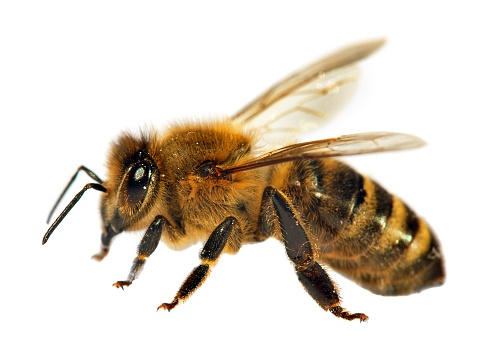
\includegraphics{immagini/capitolo1/apisMellifera.png}
    \caption{Esemplare adulto di Apis Mellifera}
    \label{fig:Apis Mellifera}
\end{figure}

\section{Docking Molecolare}
Il docking molecolare è una tecnica computazionale che mira a determinare le migliori conformazioni adottate da una molecola per legarsi ad un’altra al fine di formare un complesso stabile. Il docking molecolare viene fondamentalmente utilizzato per la valutazione delle interazioni ligando-target. A partire quindi da un ligando e dalla struttura nota del suo target, il docking molecolare permette di generare una serie di conformazioni possibili del ligando stesso localizzato all’interno del sito attivo della proteina. Esse sono denominate \textit{“binding poses”} e sono valutate da particolari funzioni chiamate \textit{“scoring functions”}, che creano quindi un vero e proprio ranking. Le \textit{migliori poses} rappresentano quella che viene identificata come la miglior soluzione proposta dall’algoritmo per l’interazione tra il ligando e il target\cite{meng2011molecular}.\newline
Gli algoritmi di docking sono formati da due componenti fondamentali:

\begin{itemize}
    \item L’algoritmo di ricerca o \textit{“search algorithm”}
    \item La \textit{“scoring function”}.
\end{itemize} 

Il primo si occupa di generare un insieme di 12 conformazioni del ligando all’interno del sito designato del target, mentre la seconda valuta le \textit{poses} generate, assegnando a ciascuna di esse un punteggio detto \textit{“score”} in base a parametri di tipo geometrico ed energetico. Le migliori conformazioni in uscita da questa valutazione sono passate nuovamente all’algoritmo di ricerca, che andrà a creare una nuova generazione di conformazioni partendo dalle migliori soluzioni dell'esecuzione precedente. Il funzionamento iterativo del \textit{search algorithm} e della \textit{scoring function} permettono di ottenere, alla fine di un determinato numero di cicli, un insieme di \textit{poses} che vengono fornite come output all’utente e che sono ritenute essere le migliori soluzioni per il \textit{binding} delle molecole in esame da parte del programma di docking utilizzato.\newline
In generale, il docking molecolare è eseguibile in tre differenti condizioni, che si differenziano l’una dall’altra per i gradi di libertà tenuti in considerazione dall’algoritmo durante il calcolo: 

\begin{enumerate}[label=\Roman{*}., ref=(\Roman{*})]
    \item \textbf{docking a corpo rigido}, che approssima sia il ligando che la proteina come strutture rigide
    \item \textbf{docking semi-flessibile}, che considera il target come rigido, tendendo però in considerazione i gradi di libertà conformazionale del ligando
    \item \textbf{docking flessibile}, in cui vengono considerati i gradi di libertà sia del ligando che dei residui del target nel sito attivo.
\end{enumerate}

Intuitivamente, passando da un approccio a corpo rigido fino ad uno flessibile, la complessità di calcolo aumenta, e proporzionalmente, anche il tempo di esecuzione.\newline
Ad oggi sono disponibili diversi protocolli di docking ognuno dei quali sfrutta una particolare coppia algoritmo di \textit{ricerca-scoring function}.\newline
Il docking molecolare consiste in tre obiettivi principali collegati tra loro: 

\begin{enumerate}[label=\arabic{*}., ref=(\arabic{*})]
    \item predizione della posa
    \item screening virtuale
    \item stima dell'affinità di legame.
\end{enumerate}

Una metodologia di docking di successo deve essere in grado di prevedere correttamente la posa nativa del ligando all'interno del sito di legame del recettore, cioè trovare la geometria sperimentale del ligando entro un certo limite di tolleranza, e le interazioni fisico-chimiche molecolari associate.\newline
Quando si analizzano librerie di composti di grandi dimensioni, il metodo deve essere in grado di distinguere con successo le molecole che si legano da quelle che non si legano e di classificare correttamente questi ligandi tra i migliori composti del database.\newline
Un algoritmo di ricerca e una funzione di score energetico sono gli strumenti di base di una metodologia di docking per generare e valutare le conformazioni dei ligandi. La capacità di gestire con successo la flessibilità molecolare intrinseca di un sistema e di descrivere correttamente l'energia delle interazioni recettore-ligando è cruciale per lo sviluppo di metodologie di docking predittivo che sono utili negli studi prospettici di progettazione di farmaci\cite{guedes2014receptor}.

\begin{figure}[H]
    \centering
    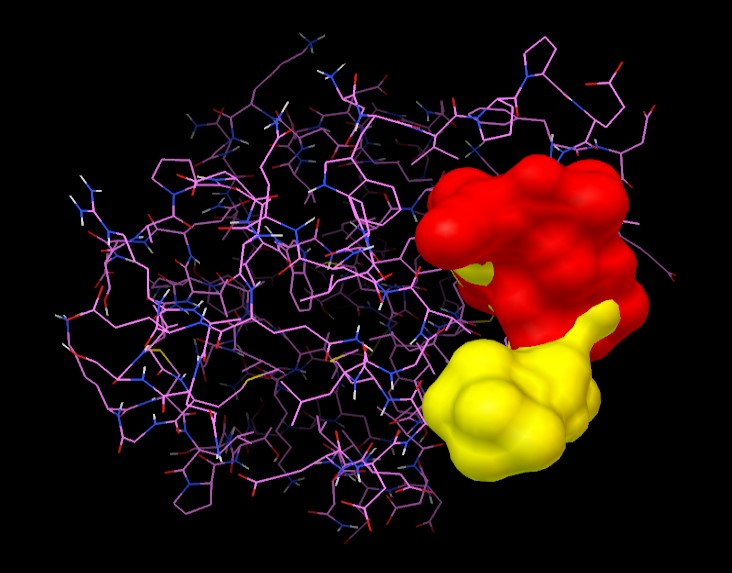
\includegraphics{immagini/capitolo1/dockingMolecolare.png}
    \caption{Rappresentazione del docking tra il ligando acrinathrin e la proteina 2h8v}
    \label{fig:docking molecolare}
\end{figure}

\section{Simulazione}
La \textbf{simulazione} di un processo di docking è un processo molto più che complicato. In tale approccio, la proteina e il ligando sono separati fisicamente da una certa distanza, e il ligando trova la sua posizione nel sito attivo della proteina dopo aver compiuto diversi movimenti nello spazio. Tali movimenti includono rotazioni, traslazioni e torsione di alcuni angoli di rotazione degli atomi. Ognuno di questi movimenti ha un determinato costo energetico nel sistema, dato che dopo ogni mossa viene ricalcolata l'energia totale. Questo approccio rappresenta molto bene quello che accade nella realtà. Di contro, il costo richiesto in termini di tempo e prestazioni è molto elevato.
    
\section{Software per il docking molecolare}
I programmi di docking molecolare eseguono un algoritmo di ricerca in cui la conformazione del ligando viene valutata ricorsivamente fino a raggiungere la convergenza all'energia minima. Infine, una funzione di punteggio di affinità, $\Delta$G (Energia potenziale totale in kcal/mol), viene impiegata per classificare le pose candidate come la somma delle energie elettrostatiche e di van der Waals. Le forze trainanti per queste specifiche interazioni nei sistemi biologici mirano alla complementarità tra la forma e l'elettrostatica delle superfici del sito di legame e del ligando o del substrato. \newline
Negli ultimi vent'anni, sono stati sviluppati più di 60 diversi strumenti e programmi di docking sia per uso accademico e commerciali, come DOCK (Venkatachalam et al. 2003), AutoDock (Österberg et al. 2002), FlexX (Rarey et al. 1996), Surflex (Jain 2003), GOLD (Jones et al. 1997), ICM (Schapira et al. 2003), Glide (Friesner et al. 2004), Cdocker, LigandFit (Venkatachalam et al. 2003), MCDock, FRED (McGann et al. 2003), MOE-Dock (Corbeil et al. 2012), LeDock (Zhao e Caflisch 2013), AutoDock Vina (Trott e Olson 2010), rDock (Ruiz-Carmona et al. 2014), UCSF Dock (Allen et al. 2015) e molti altri. \newline 
Tra questi programmi, AutoDock Vina, GOLD e MOE-Dock hanno predetto le pose migliori con gli score migliori. AutoDock e LeDock sono stati in grado di identificare i corretti legami dei ligandi nelle pose. Sia Glide (XP) che AutoDock hanno previsto le pose con un'accuratezza del 90,0\% (Wang et al. 2016). È stato dimostrato che AutoDock ha prodotto fattori di arricchimento più rispetto a Glide in uno studio di screening virtuale contro il Fattore Xa, mentre Glide ha superato AutoDock contro lo stesso bersaglio in un analogo studio di screening virtuale. Nel complesso, è stato riportato recentemente che questi programmi di docking sono in grado di predire pose sperimentali con deviazioni al quadrato della radice (RMSD) in media (RMSD) in media da 1,5 a 2 Å\cite{pagadala2017software}.\newline 
Come mostrato nella Figura 1.3, il software di docking molecolare può aiutarci a individuare la conformazione e l'orientamento ottimali in base alla complementarità e alla pre-organizzazione con un algoritmo specifico, quindi ad applicare una funzione di scoring per prevedere l'affinità del legame e ad analizzare la modalità interattiva\cite{fan2019progress}.

\begin{figure}[H]
    \centering
    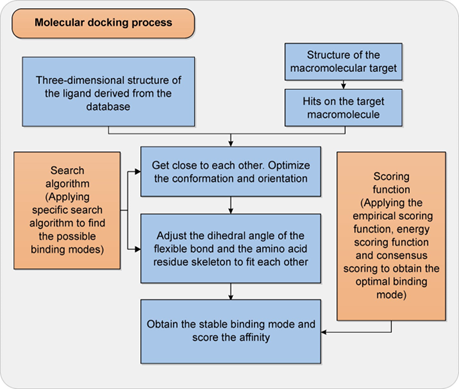
\includegraphics{immagini/capitolo1/processoDockingMolecolare.png}
    \caption{Processo del docking molecolare}
    \label{fig:processo del docking Molecolare}
\end{figure}

\section{Gestione del lavoro}
Il software trattato è frutto del lavoro congiunto del sottoscritto e del mio collega di studi Massimiliano Giordano Orsini con il coordinamento del ricercatore del CNR dottor Ferdinando Febbraio. Il lavoro per quanto prodotto e per il suo svolgimento può essere considerato alla stregua di un progetto software vero e proprio. Sono stati necessari diversi incontri con il dottor Febbraio in quanto esperto del \textbf{dominio applicativo} per chiarire concetti poco familiari, a me ed al mio collega, dell'ambito in cui l'applicazione andava sviluppata: la biologia.\newline 
Dopo varie fasi di \textbf{analisi} e di \textbf{progettazione} si è passato alla fase di \textbf{sviluppo} corrispondente alla fase di effettiva implementazione del software. Infine sono state effettuate le fasi di \textbf{testing} funzionale (FAT) e utente (UAT), nell'ultima fase ha partecipato il dottor Febbraio, per individuare e risolvere errori e bug ed approvare il software realizzato. Le varie fasi di sviluppo software non si sono succedute in maniera sequenziale, seguendo quindi i dettami del modello di sviluppo \textbf{waterfall}, bensì le varie fasi sono state inframmezzate l'una con l'altra e, più che come passi di un processo sono state iterazioni cicliche delle stesse, rispettando i paradigmi dello sviluppo \textbf{agile}.\newline
Questo processo di sviluppo è stato dettato dalla natura stessa del progetto, poiché a seguito del repentino raggiungimento con successo degli obbiettivi prefissati, sono sopravvenute ulteriori richieste di implementazioni per dotare di maggiore complementarietà il software prodotto.

\section{Idea e sviluppo}
L’\textbf{idea} nasce dall’attività di tirocinio svolta presso il "Consiglio Nazionale di Ricerca" di Napoli, per un totale di 300 ore, sotto la supervisione del Responsabile del laboratorio di informatica dell'università Parthenope, professor Angelo Ciaramella e del dottore Ferdinando Febbraio del CNR di Napoli. Il lavoro effettuato è consistito nella realizzazione di un software, del tutto preliminare al progetto di tesi proposto. Lo \textbf{sviluppo} è avvenuto attraverso diverse fasi nelle quali sono stati utilizzati ed implementati i seguenti tools: 

\begin{itemize}
    \item software per l'esecuzione del docking
    \item funzioni di bioinformatica per la preparazione degli input necessari
    \item software per l'analisi dei risultati dell'intero processo.
\end{itemize}

Sono state determinate le componenti software ideali per automatizzare il processo di docking conseguendo risultati efficienti per quanto riguarda l'output e l'analisi dello stesso, offrendo una buona usabilità del prodotto realizzato mediante una semplice ed intuitiva interfaccia grafica.

\section{Descrizione dell'applicazione}
Il progetto di tesi proposto ha come focus principale la realizzazione di un applicativo che effettua il docking tra i ligandi contenuti in specifici pesticidi e i recettori dell’ Apis mellifera e l’estrazione dei legami che si vengono a 
formare.\newline
Il nome scelto per l'applicazione realizzata è \textbf{Computational Docking} in quanto prova della digitalizzazione della disciplina biologica.\newline
L’applicazione può essere scaricata con le configurazioni di default, direttamente dalla repository di github. Il software realizzato può essere utilizzato in due modalità: 

\begin{itemize}
    \item mediante \textbf{script python da terminale}
    \item mediante \textbf{interfaccia grafica} realizzata seguendo il paradigma model ViewController.
\end{itemize} 

La GUI usufruirà degli stessi script lanciati da riga di comando garantendo le stesse funzionalità secondo i dettami della OOP, ossia riutilizzo del codice funzionante anziché modifiche dello stesso o scriverne uno nuovo.\newline
L’applicazione è composta da tre \textbf{moduli}:

\begin{enumerate}
    \item Preparazione dei ligandi e dei recettori
    \item Esecuzione del docking
    \item Analisi dei risultati del docking.
\end{enumerate}

\begin{figure}[H]
    \centering
    
\includegraphics[scale=0.1]{immagini/capitolo1/QRcode.png}
    \caption{QR code della repository di GitHub di Computational Docking}
    \label{fig:QR code}
\end{figure}

\section{Contenuto della tesi}
La tesi è divisa in tre moduli:

\begin{enumerate}
    \item nel primo modulo saranno discusse le tecnologie, le piattaforme scelte per la realizzazione del software, i linguaggi di programmazione e gli strumenti di bioinformatica utilizzati
    \item nel secondo modulo sarà illustrata l'applicazione realizzata, dalla preparazione dei ligandi e recettori, passando per il docking, finendo con l'estrazione dei legami dall'output ottenuto
    \item nell'ultimo modulo saranno trattate le conclusioni e saranno indicati gli sviluppi futuri del software realizzato.
\end{enumerate} 

\begin{figure}[H]
    \centering
    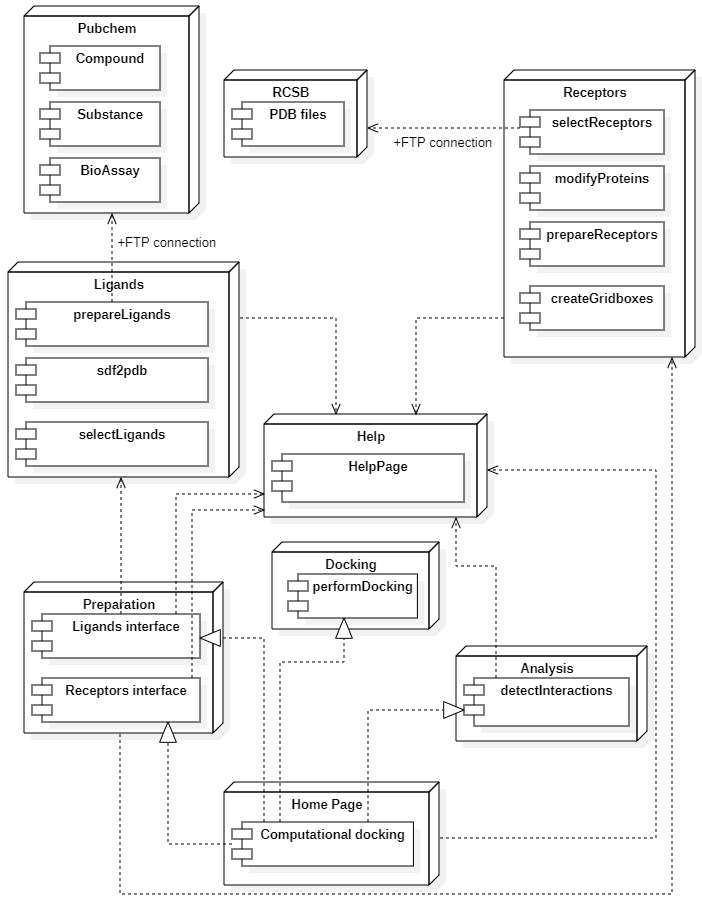
\includegraphics[scale=0.9]{immagini/capitolo1/UML.png}
    \caption{Diagramma implementativo del software}
    \label{fig:UML}
\end{figure}
    \def\baselinestretch{1}
\chapter{Tecnologie e piattaforme} \label{cap2}
\def\baselinestretch{1.66}

\def\baselinestretch{1.66}
\noindent In questo capitolo verranno trattate le tecnologie utilizzate, a partire dai linguaggi, i tools utilizzate e le piattaforme hardware di lavoro. È stato fondamentale l’utilizzo di macchine in remoto per eseguire le operazioni di training del modello. In questo caso le macchine messe a disposizione dall’Università Parthenope e dal CNR sono state fondamentali in quanto hanno garantito stabilità ed efficienza.

\section{Linguaggi e tools}
\def\baselinestretch{1.66}
\noindent La scelta del linguaggio di programmazione è stata importante in quanto ci sono tantissimi linguaggi con librerie adatte allo scopo, solo pochi ricevono costante supporto e sono anche utilizzati nel mondo del lavoro.

\subsection{Python}
\def\baselinestretch{1.66}
\noindent \textbf{Python} è un linguaggio di programmazione dinamico orientato agli oggetti utilizzabile per molti tipi  di sviluppo software. Offre un forte supporto all'integrazione con altri linguaggi e programmi, è fornito di una estesa libreria standard e può essere imparato in pochi giorni. Python inoltre è fornito delle librerie di bioinformatica adatte allo scopo del software realizzato. Di seguito le principali utilizzate:
\begin{itemize}
    \item \textbf{pubchempy}, per le ricerche chimiche per nome, sottostruttura e somiglianza, standardizzazione chimica, conversione tra formati di file chimici, rappresentazione e recupero delle proprietà chimiche
    \item \textbf{prody}, per l'analisi della dinamica strutturale delle proteine
    \item \textbf{pandas}, per la manipolazione ed analisi dei dati
    \item \textbf{customTkinter}, per la realizzazione dell'interfaccia grafica
    \item \textbf{MolKit}, pacchetto che fornisce classi per leggere le molecole in diversi formati di file (PDB, Mol2...) e costruire una struttura gerarchica ad albero che riproduce la struttura interna della molecola
    \item \textbf{Matplotlib}, per la creazione di visualizzazioni statiche, animate e interattive
    \item \textbf{customTkinter}, per la realizzazione dell'interfaccia grafica
    \item \textbf{numpy}, per la gestione delle strutture dati
    \item \textbf{os}, per la gestione dei files
\end{itemize} 
La versione di Python utilizzata è la \textbf{2.7} in quanto maggiormente compatibile con le librerie e i pacchetti utilizzati.

\subsection{ADFRsuite}
\def\baselinestretch{1.66}
\noindent \textbf{AutoDockFR} (o \textbf{ADFR} in breve) è un programma per il \textbf{docking tra proteine e ligandi} sviluppato nel laboratorio Sanner dello Scripps Research sotto l'egida di \textit{AutoDock}.\newline
Utilizza:
\begin{itemize}
    \item la funzione di scoring di \textit{AutoDock4}, implementata in una libreria C++ ed inglobata in Python
    \item un proprio algoritmo genetico in grado di evolvere e ottimizzare più soluzioni simultaneamente, di gestire un gran numero di legami ruotabili e di terminare le iterazioni al momento della convergenza, cioè potenzialmente senza esaurire il numero assegnato di valutazioni della funzione energia
    \item una rappresentazione generica di flessibilità molecolare, chiamata \textit{Albero di Flessibilità}, che consente di incorporare una varietà di movimenti molecolari sia nel ligando che nel recettore.
\end{itemize}
Pur supportando le modalità di docking disponibili in \textit{AutoDock4} e \textit{Vina}, è stato progettato specificamente per includere la \textbf{flessibilità del recettore} e supporta anche il \textbf{docking covalente}. Il suo algoritmo genetico personalizzato consente il docking di ligandi con più legami ruotabili rispetto ad \textit{AutoDock4}.\newline
Viene distribuito come parte della suite del software \textit{ADFR}, che fornisce strumenti aggiuntivi per facilitare il docking automatizzato.\newline
\textit{ADFR} implementa diverse caratteristiche che aiutano a semplificare la procedura di docking e a supportare la gestione e la riproducibilità degli esperimenti di docking attraverso la prova dei dati. Vengono utilizzati file autodocumentati per memorizzare: 
\begin{itemize}
    \item la rappresentazione del sito di binding (cioè \textbf{i file .trg target})
    \item i risultati del docking (file \textbf{.dro Docking Results Object})
    \item I metadati memorizzati in questi file non solo supportano la riproducibilità, ma riducono anche i rischi di errori dell'operatore.
\end{itemize}
\noindent ADFR legge i \textbf{ligandi} preparati per il docking con AutoDock, cioè nel formato PDBQT e organizza la flessibilità del ligando in base ai legami ruotabili. Un file PDBQT può essere generato da un file .pdb di un ligando utilizzando il comando \textit{prepar\_ligand}.  Il \textbf{recettore} è specificato come file target, cioè un singolo file che descrive il recettore. I file target possono essere calcolati per un recettore nel formato PDBQT dal comando utilizzando il programma \textit{\textbf{agfr}} o l'interfaccia grafica \textit{\textbf{agfrgui}}. Un file PDBQT può essere generato da un file pdb di un recettore utilizzando il comando \textit{prepare\_receptor} della suite \textit{ADFR}. \newline
\textit{ADFR} è implementato nei moderni linguaggi di programmazione orientati agli oggetti e si basa su componenti software riutilizzabili. I componenti critici per le prestazioni sono implementati in C e C++ (ad esempio ADFRcc), mentre altri sono implementati in Python (ADFR, AutoSite, MolKit2, prody). \textit{ADFR} è rilasciato sotto la licenza open source LGPL v2.\newline 
In particolare per l'applicazione trattata sono stati utilizzati i due script: \textbf{prepare\_ligand4} e \textbf{prepare\_receptors4}, rispettivamente per la preparazione dei ligandi e dei recettori e per effettuare la loro conversione dal formato .pdb al formato .pdbqt necessario per la procedura di docking.

\subsection{MGLTools}
\def\baselinestretch{1.66}
\noindent La suite software \textbf{MGLTools} è stata sviluppata nel laboratorio Sanner presso il Center for Computational Structural Biology (CCRB) precedentemente noto come Molecular Graphics Laboratory (MGL) dello Scripps Research Institute per la visualizzazione e l'analisi delle strutture molecolari. MGLTools comprende:
\begin{itemize}
    \item \textbf{Python Molecular Viewer (PMV)}, un visualizzatore molecolare di uso generale
    \item \textbf{AutoDockTools (ADT)}, un insieme di comandi PMV sviluppati specificamente per supportare gli utenti di AutoDock
    \item \textbf{Vision}, un ambiente di programmazione visuale.
\end{itemize}
\noindent Questi strumenti software sono altamente integrati e basati su componenti software riutilizzabili implementati in Python e C++ (con binding Python). Il kit di strumenti grafici sottostante è Tk (Tkinter).L'ultima versione di MGLtools è la 1.5.7 che fornisce:
\begin{itemize}
    \item un widget della dashboard ridisegnato
    \item un widget per la visualizzazione delle sequenze
    \item ottimizzazioni delle prestazioni
    \item nuovi comandi per i calcoli di sovrapposizione e RMSD
\end{itemize}

\subsection{Open Babel}
\def\baselinestretch{1.66}
\noindent \textbf{Open Babel} è un tool per applicazioni di chimica progettato per interpretare i molteplici formati dei dati chimici e per cercare, convertire, analizzare o archiviare dati da modellistica molecolare, chimica, materiali a stato solido, biochimica o aree correlate.\newline
La versione di OpenBabel 2.3 converte fino a 110 formati di file chimici.\newline
I database sono ampiamente utilizzati per memorizzare le informazioni chimiche soprattutto nell'industria farmaceutica. Un requisito fondamentale di un database di questo tipo è la capacità di indicizzare le strutture strutture chimiche in modo che possano essere recuperate rapidamente, data una quary di ricerca. Open Babel offre questa funzionalità utilizzando un'indicizzazione basata sul percorso. Questa indicizzazione, FP2 in Open Babel, identifica tutte le sottostrutture lineari e ad anello della molecola di lunghezza da 1 a 7 (escluse le sottostrutture a 1 atomo C e N) e le mappa in una stringa di bit di lunghezza su una stringa di bit di lunghezza 1024 utilizzando una funzione di hash. Se una molecola interrogata è una sottostruttura di una molecola di destinazione, tutti i bit molecola di destinazione, allora tutti i bit impostati nella molecola di query saranno impostati anche nella molecola di destinazione. Le indicizzazioni
di due molecole possono anche essere utilizzate per calcolare la somiglianza strutturale utilizzando il coefficiente di Tanimoto, il numero di bit in comune diviso per tutti i bit dell'insieme.
Chiaramente, la ricerca iterativa dello stesso insieme di molecole comporterà l'uso ripetuto dello stesso insieme di indicizzazioni. Per evitare la necessità di ricalcolare le indicizzazioni per un particolare file multi-molecola (come un file SDF), Open Babel fornisce un formato fastindex che memorizza esclusivamente un'indicizzazione insieme a un indice nel file originale. Questo indice porta a un rapido aumento della velocità di ricerca di corrispondenze a a fronte di una quary: insiemi di dati con diversi milioni di molecole sono facilmente consultabili in modo interattivo. In questo in questo modo, un file multi-molecola può essere utilizzato come un'alternativa efficace a un sistema di database chimico \cite{o2011open}.

\section{Database}
\def\baselinestretch{1.66}
\noindent \textbf{PubChem} è il più grande database al mondo di informazioni chimiche liberamente accessibili, attraverso il quale è possibile cercare le sostanze chimiche per nome, formula molecolare, struttura e altri identificatori. Inoltre è possibile trovare proprietà chimiche e fisiche, attività biologiche, informazioni sulla sicurezza e sulla tossicità, brevetti, citazioni bibliografiche e altro ancora. L'interfaccia tra l'applicazione ed il database è realizzata mediante la libreria di Python \textbf{pubchempy}.\newline
PubChem è un database di molecole chimiche, gestito dal centro nazionale per l'Informazione biotecnologica statunitense (NCBI), parte della biblioteca nazionale di medicina (NLM) dell'istituto nazionale della sanità americano (NIH). L'accesso al database PubChem può essere eseguito liberamente attraverso un sito web e possono essere scaricati dati riguardanti milioni di strutture di composti e dati descrittivi tramite il protocollo FTP.PubChem possiede descrizioni di molecole con meno di 1000 atomi e 1000 legami. \newline 
PubChem gestisce i dati in tre database interconnessi: \textbf{Substance, Compound e BioAssay}. Il database Substance archivia le descrizioni delle sostanze chimiche fornite dai depositanti. Il database Compound archivia le strutture chimiche uniche estratte dal database Substance attraverso la standardizzazione delle strutture. Il database BioAssay contiene la descrizione e i risultati degli esperimenti di analisi biologica.

\section{Autodock}
\def\baselinestretch{1.66}
\noindent \textbf{AutoDock} è un programma di docking che utilizza un algoritmo genetico, il \textit{Lamarckian Genetic Algorithm}, per il calcolo della pose migliore che interagisce con il sito attivo della proteina. Dopo aver calcolato inizialmente una popolazione di possibili soluzioni, l’algoritmo ne selezionerà una parte in base alle funzioni di scoring e darà origine a una nuova popolazione di soluzioni figlie, da cui avrà inizio un secondo ciclo di generazione e così via. In questo modo il “genotipo”, ovvero la stringa binaria a cui corrisponde ciascun ligando, verrà influenzato da fattori esterni, esattamente come nell’ipotesi lamarckiana.\newline
Le popolazioni di soluzioni sono ottenute tramite operatori genetici (mutazioni, crossover e migrazioni) che imitano quelli biologici. I gradi di libertà sono codificati in geni o stringhe binarie, e a geni e cromosomi è assegnato un valore basato sulla fitness della scoring function. Le operazioni di mutazione causano cambiamenti nel valore di un gene, mentre il crossover muove un set di geni da un cromosoma “genitore” ad un altro; la migrazione invece muove singoli geni da una sottopopolazione ad un’altra.\newline
L’interazione tra ligando e recettore è valutata in due fasi, calcolando la variazione di energia intramolecolare del passaggio dalla forma libera a quella legata e la variazione di energia libera intermolecolare implicata nello stesso passaggio.\newline
Per effettuare il docking è necessario per prima cosa preparare le coordinate di ligando e recettore. La preparazione delle coordinate è la fase più importante nella procedura, poiché in esse sono inclusi parametri fondamentali come: idrogeni polari, atom – type e cariche parziali. Le coordinate del ligando originale e della macromolecola sono trattate separatamente ed i loro file sono in un formato particolare, il PDBQT.

\section{Autodock Vina}
\def\baselinestretch{1.66}
\noindent \textbf{AutoDock Vina} è  un nuovo programma per il docking molecolare e lo screening virtuale. Vina rappresenta la nuova versione di AutoDock, ed infatti presenta molte similitudini con il suo predecessore ma, allo stesso tempo, anche molte differenze. Una differenza importante consiste nella velocità di calcolo, dato che Vina è molto poco dispendioso sotto questo punto di vista; altra differenza fondamentale è rappresentata dal fatto che al momento del calcolo della griglia, Vina calcola internamente ed automaticamente le “grid maps” impiegate in AutoDock. Questo costituisce un grande vantaggio in termini di facilità e velocità di esecuzione. Inoltre, le funzioni di scoring e gli algoritmi utilizzati in questo tipo di analisi risultano essere completamente diversi rispetto al suo predecessore, cosa che porta a considerare Vina quasi come un software a sé stante. Vina migliora al tempo stesso in modo significativo l'accuratezza delle previsioni delle modalità di legame. Un'ulteriore miglioramento è ottenuta grazie al parallelismo, che utilizza il multithreading su macchine multicore. AutoDock Vina calcola automaticamente le mappe della griglia e raggruppa i risultati in modo trasparente per l'utente. Autodock vina all'interno del software prende in input i ligandi ed i recettori in formato .pdbqt.

\subsection{Funzione di scoring}
\def\baselinestretch{1.66}
\noindent La funzione di scoring di AutoDock Vina (qui indicata come Vina) può essere rappresentata attraverso la seguente formula:\newline
\begin{equation}
    c = \sum_{i<j}f_{t_it_j}(r_{ij})
\end{equation} \newline
dove la sommatoria è su tutte le coppie di atomi che possono muoversi l'uno rispetto all'altro, escludendo normalmente le interazioni 1-4, ovvero gli atomi separati da tre legami covalenti consecutivi. Ad ogni atomo $i$ viene assegnato un tipo $t_i$ e un insieme simmetrico di funzioni di interazione $f_{t_it_j}$ della distanza interatomica $r_{ij}$ da definire.\newline
Questo valore può essere visto come una somma di contributi intermolecolari e intramolecolari:\newline
\begin{equation}
    c = c_{inter} + c_{intra}
\end{equation}\newline
L'algoritmo di ottimizzazione, descritto in seguito, cerca di trovare il minimo globale di $c$ e di altre conformazioni a basso punteggio, che poi classifica.\newline 
L'energia libera di legame prevista viene calcolata a partire dalla parte intermolecolare della conformazione con il punteggio più basso, designata come:\newline
\begin{equation}
    s_1 = g(c_1 - c_{intra1}) = g(c_{inter1})
\end{equation}\newline
dove la funzione $g$ può essere una funzione arbitraria strettamente crescente possibilmente non lineare.\newline Nell'output le altre conformazioni a basso punteggio vengono formalmente restituite dai valori di $s$, ma per preservare il ranking, si utilizza $c_{intra}$ come migliore modalità di legame:\newline
\begin{equation}
    s_i = g(c_i - c_{intra1})
\end{equation}\newline
Per ragioni di modularità, gran parte del programma non fa riferimento ad alcuna forma funzionale delle interazioni $f_{t_it_j}$ o $g$. Essenzialmente, queste funzioni vengono passate come parametro per il resto del codice. Inoltre, il programma è stato progettato in modo tale da poter utilizzare schemi di tipizzazione degli atomi come la tipizzazione degli atomi di AutoDock4 o SYBIL.\newline
\begin{table}[H]
    \centering
    \begin{tabular}{|l|l|}
        \hline
        \textbf{Pesi} & \textbf{Termini}\\
        \hline
        $-0.0356$ & $gauss_1$\\
        $-0.00516$ & $gauss_2$\\
        $0.840$ & $repulsion$\\
        $-0.0351$ & $hydrophobic$\\
        $-0.587$ & $hydrogen bonding$\\
        $0.0585$ & $N_{rot}$\\
        \hline
    \end{tabular}
    \caption{Funzione di scoring pesi e termini}
    \label{tab:Tabella Pesi e Termini}
\end{table}
\noindent La particolare implementazione della funzione di scoring che verrà presentata è stata ispirata principalmente da X-score e come tale è stato messo a punto utilizzando PDBbind. Tuttavia, alcuni termini sono diversi da X-score e, nel mettere a punto la funzione di scoring, si è andati oltre la regressione lineare. Inoltre, va notato che Vina classifica le conformazioni secondo l'eq. (2.2) o, equivalentemente, eq. (2.4), mentre X-score conta solo i contributi intermolecolari.
Per quanto ne sappiamo, X-score non è stato implementato in un programma di docking, ignorare i vincoli interni potrebbe portare l'algoritmo di ottimizzazione a ricercare strutture corrotte all'interno.\newline
La derivazione della nostra funzione di scoring combina alcuni vantaggi tra quelli potenzialmente conosciuti e le funzioni di scoring empiriche: estrae informazioni empiriche da entrambe le preferenze conformazionali del sia dei complessi recettore-ligando sia dalle misure sperimentali affini.\newline 
Lo schema di tipizzazione degli atomi segue quello di X-score. Gli atomi di idrogeno non sono considerati esplicitamente, se non per la tipizzazione degli atomi, e sono omessi dall'eq. (2.1).\newline
Le funzioni di interazione $f_{t_it_j}$ sono definite rispetto alla distanza di superficie  $d_{ij} = r_{ij} - R_{ti}
- Rtj$:\newline
\begin{equation}
    f_{t_it_j}(r_{ij}) \equiv h_{t_it_j}(d_{ij})
\end{equation}\newline
dove $R_t$ è il raggio di van der Waals dell'atomo di tipo $t$.\newline
Nella nostra funzione di scoring, $h_{t_it_j}$ è una somma ponderata di interazioni steriche (i primi tre termini nella tabella 2.1), identica per tutte le coppie di atomi, interazione idrofobiche tra atomi idrofobici e, dove possibile, legami a idrogeno. I pesi sono mostrati nella tabella 2.1. I termini sterici sono i seguenti:\newline
\begin{equation}
    gauss_1(d)=e^{-(d/0.5\mathring{A})^2}
\end{equation}
\begin{equation}
    gauss_2(d)=e^{-((d/0.5\mathring{A})/2\mathring{A})^2}
\end{equation}
\begin{equation}
    repulsion(d) = \begin{cases}
                        d^2, se & d < 0\\
                        0, se & d \geq 0
                    \end{cases}
\end{equation}\newline
Il termine idrofobico è uguale a $1$, quando $d < 0,5\mathring{A}$; $0$, quando $d > 1,5\mathring{A}$, ed è interpolato linearmente tra questi valori. Il termine di legame a idrogeno è uguale a $1$, quando $d < -0,7\mathring{A}$; $0$, quando $d < 0,5\mathring{A}$, e viene interpolato linearmente tra questi valori. Seguendo Xscore, trattiamo formalmente i metalli come donatori di legami a idrogeno. In questa in questa implementazione, tutte le funzioni di interazione $ f_{t_it_j}$ sono tagliate a $r_{ij} = 8\mathring{A}$.\newline
La Figura 1 mostra i termini sterici ponderati da soli o combinati con i termini idrofobici o H
con le interazioni idrofobiche o di legame H\cite{trott2010autodock}.

\begin{figure}[H]
    \centering
    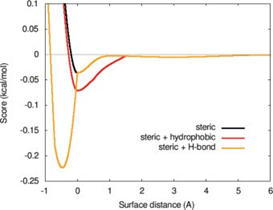
\includegraphics{immagini/funzioneScoringPesata.png}
    \caption{Funzione di scoring pesata}
    \label{fig:Funzione di scoring pesata}
\end{figure}

    \chapter{Applicazione realizzata}
L'applicazione realizzata, \textbf{Computational Docking}, effettua il docking tra i ligandi contenuti in specifici pesticidi e i recettori dell'Apis mellifera, infine effettua l'estrazione dei legami che si vengono a formare. 

\section{Installazione}
L'applicazione viene scaricata dalla \href{https://github.com/mungowz/Computational-Docking.git}{repository di github} mediante il comando:

\begin{lstlisting}[language=Bash, label=lst:code1, caption={Comando per scaricare la repository}]
git clone https://github.com/mungowz/Computational-Docking.git
\end{lstlisting}

Verrà quindi installata nella directory corrente la repository contenente il progetto, all'interno di questa si trovano gli script utilizzati dall'applicazione e le directory ed i file di input di default, tra cui:

\begin{itemize}
    \item Il file di input dei ligandi, ovvero \textit{ligands\_list.txt}
    \item La directory contenente la lista di default dei ligandi, ovvero \textit{/data/files/}
    \item La directory di default che conterrà i file \textit{.xlsx} di output prodotti, ovvero \textit{/output/excel\_files}
    \item La directory di default che conterrà i file \textit{.sdf} prodotti, ovvero \textit{/data/ligands/sdf/}
    \item Le directory di default che conterranno i file \textit{.pdb} prodotti, ovvero \textit{/data/ligands/pdb/} per i ligandi e \textit{/data/proteins/pdb/} per i recettori
    \item Le directory di default che conterranno i file \textit{.pdbqt prodotti}, ovvero \textit{/data/ligands/pdbqt/} per i ligandi e \textit{/data/proteins/pdbqt/} per i recettori.
\end{itemize}

Sarà necessario installare alcune dipendenze esterne (software esterni) ed interne (librerie e pacchetti di python) per far funzionare l'applicazione, la lista delle dipendenze e la procedura di installazione è specificata nel file \textit{README} della repository di github.

\section{Modalità di utilizzo}
\textbf{Computational Docking} può essere utilizzato in due modalità:

\begin{enumerate}[label=\arabic{*}., ref=(\arabic{*})]
    \item Mediante script python da terminale
    \item Mediante interfaccia grafica realizzata seguendo il paradigma \textit{model-view-controller}.
\end{enumerate}

Non sarà necessario effettuare ulteriori installazioni per usufruire di entrambe le modalità ma bisognerà semplicemente scaricare la repository e seguire le istruzioni del \textit{README}.\newline
Per eseguire l'applicazione da riga di comando devono essere eseguiti separatamente nell'ordine i seguenti script:

\begin{itemize}
    \item \textbf{prepare\_ligands.py}
    \item \textbf{prepare\_receptors.py}
    \item \textbf{performDocking.sh}
    \item \textbf{detect\_interactions.py}
\end{itemize}

La GUI usufruirà degli stessi script eseguiti da riga di comando, garantendo così le stesse funzionalità in entrambe le modalità di utilizzo e seguendo i dettami della \textbf{OOP} secondo i quali bisogna riutilizzare codice funzionante anzichè modificarlo o scriverlo ex-novo.\newline
Per avviare la GUI deve essere digitato nel terminale il comando:

\begin{lstlisting}[language=bash, label=lst:code2, caption={Comando per avviare la GUI}]
python app.py    
\end{lstlisting}

Avviata la GUI si aprirà la home page con le seguenti opzioni:

\begin{itemize}
    \item Opzione \textbf{Preparation}: si accede alla sezione relativa alla preparazione degli input
    \item Opzione \textbf{Docking}: sarà possibile effettuare il docking
    \item Opzione \textbf{Analysis}: sarà possibile effettuare l'analisi dei risultati del docking
    \item Opzione \textbf{Help}: si accede alla sezione relativa alle informazioni utili per l'utente per l'uso del software.
\end{itemize}

\begin{figure}[H]
    \centering
    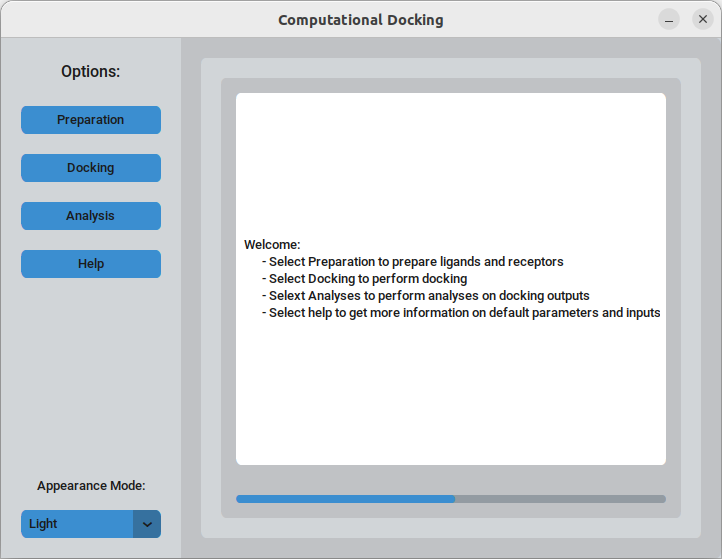
\includegraphics[scale=0.6]{immagini/capitolo3/homePage.png}
    \caption{Sezione Home Page della GUI}
    \label{fig:home page}
\end{figure}

Attraverso il menù a tendina in basso a sinistra sarà possibile scegliere il tema dell'applicazione tra:

\begin{itemize}
    \item Tema chiaro
    \item Tema scuro
    \item Tema del sistema.
\end{itemize}

\begin{figure}[H]
    \centering
    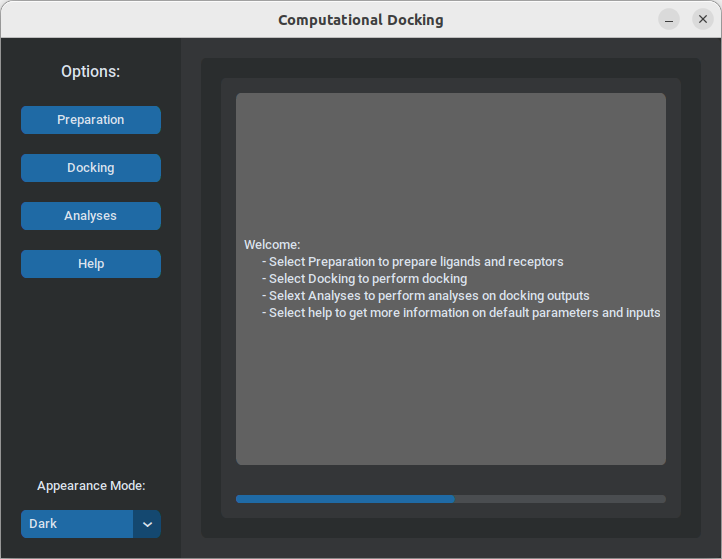
\includegraphics[scale=0.6]{immagini/capitolo3/darkGUI.png}
    \caption{Tema scuro della GUI}
    \label{fig:dark GUI}
\end{figure}

\section{Dati in input}
I dati in input all'applicazione trattata sono: ligandi e proteine.\newline
La lista dei ligandi è fornita in input tramite foglio calcolo (\textit{.xlsx}, \textit{.xls}) o mediante file di testo (\textit{.txt}), 
in entrambi i casi ogni riga corrisponde al nome di un ligando. Essendo l'applicazione incentrata sullo studio degli effetti dei ligandi dei pesticidi sull'Apis mellifera, come dati di esempio sono state utilizzati i ligandi le cui molecole costituiscono i pesticidi maggiormente diffusi sul mercato, per un totale di 297 ligandi. La lista è disponibile nell'appendice \ref{tab:Tabella dei Ligandi}.\newline
I recettori vengono selezionati mediante una \textbf{WebView} aperta sulla pagina di ricerca del sito del database \href{https://www.rcsb.org/search}{RCSB}, da qui l'utente digiterà la propria query e, dopo aver selezionato il  tasto \textbf{search} gli verranno mostrati tutti i composti organici relativi alla query digitata, tramite il tasto \textbf{Get Query} l'utente andrà a scaricare tutti i file  dei composti organici in formato \textit{.pdb}.\newline
Nel caso di esempio sono state scelte le proteine dei recettori dell'Apis Mellifera secondo la query mostrata nelle foto: \ref{fig:query recettori} e \ref{fig:file recettori}, per un totale di 11 file \textit{.pdb} contenenti le strutture di determinate proteine. La lista delle proteine scaricate è disponibile nell'appendice: \ref{Tabella dei Recettori}. L'applicazione usata tramite GUI dispone della sezione \textbf{Help} (\ref{fig:help}) contenente le informazioni relative alle impostazioni di default e al formato dei dati in input.

\begin{figure}[H]
    \centering
    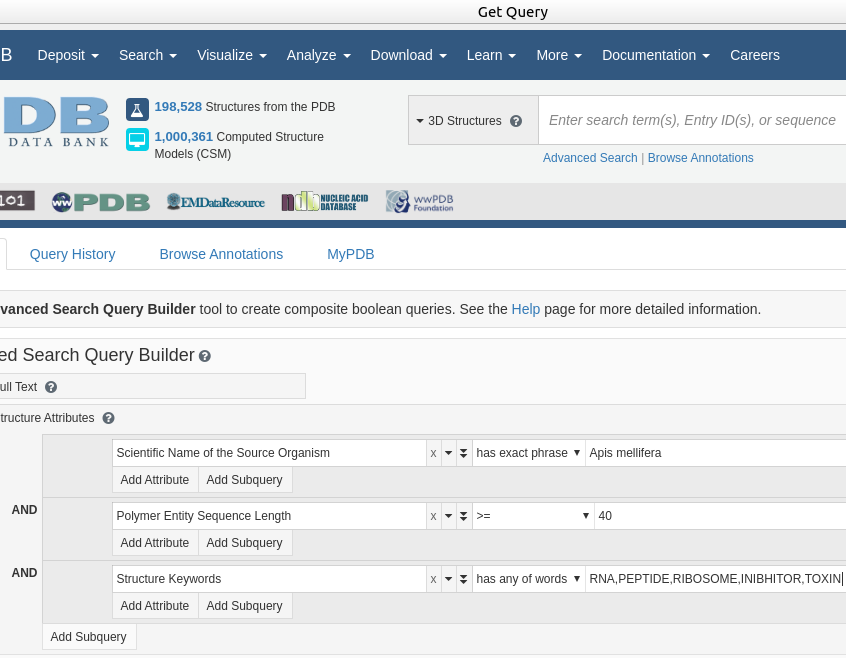
\includegraphics[scale=0.57]{immagini/capitolo3/queryRecettori.png}
    \caption{Query dei recettori}
    \label{fig:query recettori}
\end{figure}

\begin{figure}[H]
    \centering
    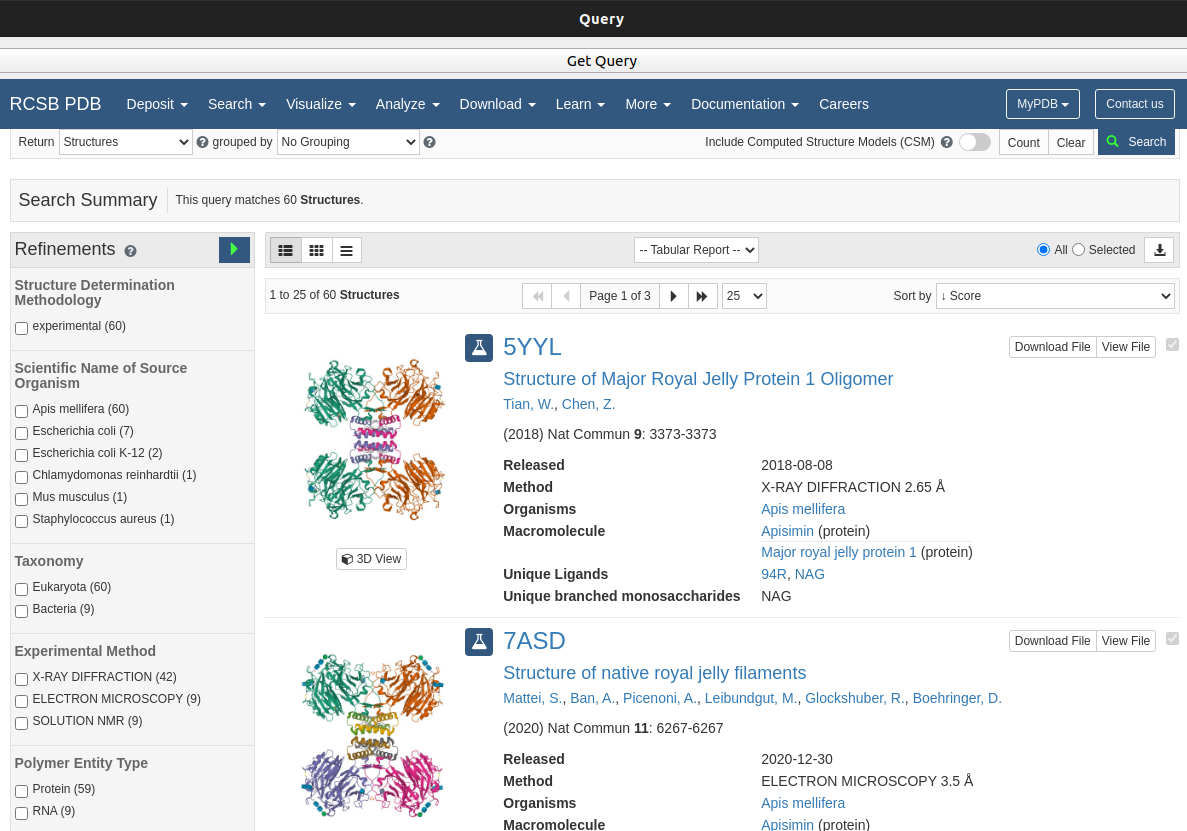
\includegraphics[scale=0.4]{immagini/capitolo3/fileRecettori.png}
    \caption{Proteine dei recettori dell'apis mellifera}
    \label{fig:file recettori}
\end{figure}

\begin{figure}[H]
    \centering
    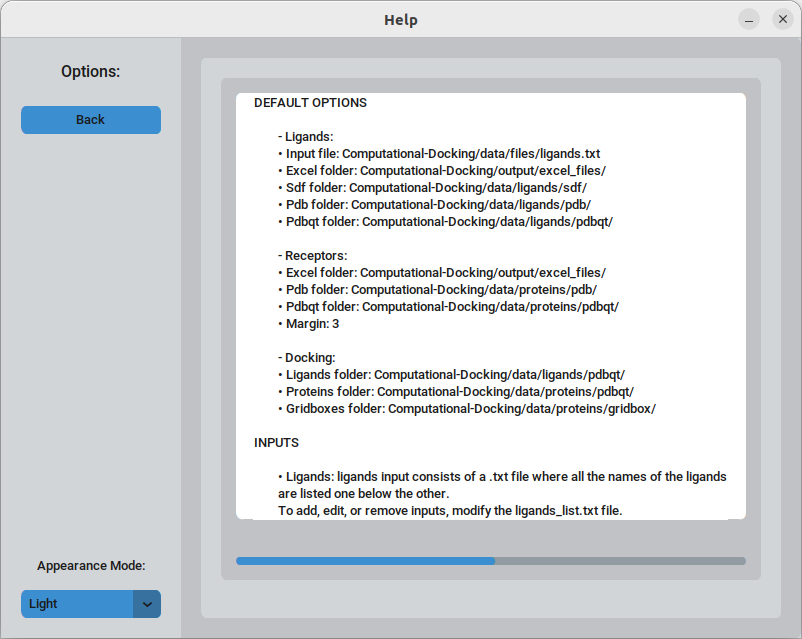
\includegraphics[scale=0.6]{immagini/capitolo3/help.png}
    \caption{Sezione Help della GUI}
    \label{fig:help}
\end{figure}

\section{Preparazione dei ligandi e recettori}
Il primo step propedeutico per il docking è la preparazione dei ligandi e dei recettori, questa
fase viene esplicitamente eseguita dal software realizzato. L'intera fase è svolta:

\begin{itemize}
    \item per i ligandi dallo script python \textbf{prepare\_ligands.py}
    \item per i recettori dallo script python \textbf{prepare\_receptors.py}.
\end{itemize}

Se l'applicazione viene utilizzata mediante GUI la preparazione dei ligandi e dei recettori può essere effettuata mediante la sezione \textbf{Preparation} della pagina principale come mostrato in figura \ref{fig:preparation}.

\begin{itemize}
    \item Selezionando l'opzione \textbf{Ligands} si accede alla sezione relativa alla preparazione dei ligandi
    \item Selezionando l'opzione \textbf{Receptors} si accede alla sezione relativa alla preparazione dei recettori
    \item Selezionando l'opzione \textbf{Back} si ritorna alla pagina principale.
\end{itemize}


\begin{figure}[H]
    \centering
    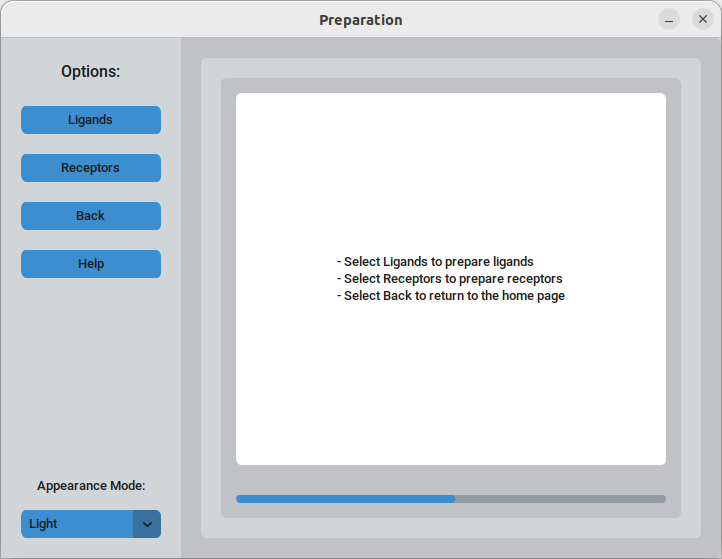
\includegraphics[scale=0.6]{immagini/capitolo3/preparation.png}
    \caption{Sezione Preparation della GUI}
    \label{fig:preparation}
\end{figure}

\subsection{Preparazione dei ligandi tramite script} \label{Preparazione dei ligandi script}
Lo script python \textbf{prepare\_ligands.py}, che esegue tale fase, viene eseguito da terminale mediante il comando:

\begin{lstlisting}[language=Bash, label=lst:code3, caption={Comando per scaricare la repository}]
python prepare_ligands.py
\end{lstlisting}

Questo script può ricevere diversi argomenti in input:

\begin{itemize}
    \item $[-v]$: serve per attivare il verbose e se non viene specificata tale opzione viene lasciata di default inattivo
    \item $[-e]$: specifica un nuovo file di input (\textit{.xlsx}, \textit{.xls}) o (\textit{.txt}) da cui prendere i nomi dei ligandi, se non viene specificata tale opzione verrà scelto il file di default scaricato insieme al software
    \item $[-E]$: specifica la directory dei file \textit{.xlsx} di output, se non viene specificata tale opzione verrà scelta la directory di default
    \item $[-s]$: specifica la directory dei file \textit{.sdf} di output, se non viene specificata tale opzione verrà scelta la directory di default
    \item $[-P]$: specifica la directory dei file \textit{.pdb} di output, se non viene specificata tale opzione verrà scelta la directory di default
    \item $[-p]$: specifica la directory dei file \textit{.pdbqt} di output, se non viene specificata tale opzione verrà scelta la directory di default
    \item $[-k]$: specificando questa opzione viene scelto di non cancellare i file dei ligandi precedentemente scaricati, se non viene specificata tale opzione i file verranno cancellati
    \item $[-h]$: stampa la spiegazione degli input per lo script.
\end{itemize}

Lo script quando eseguito andrà ad inizializzare i vari percorsi, nel caso siano stati inseriti percorsi diversi da quelli di default verrà controllata l'esistenza e la validità degli stessi. Nel caso non siano presenti le directory contenenti i file \textit{.sdf}, \textit{.pdb} e \textit{.pdbqt}, queste verranno create automaticamente dall'applicazione, inoltre verranno cancellati i file precedentemente scaricati a meno di input diversi.\newline
Lo script richiama la funzione \textbf{selectLigands} la quale si occupa di scaricare da \textbf{Pubchem}
i file \textit{.sdf} corrispondenti alla lista dei ligandi in input. La funzione prende in input: 

\begin{itemize}
    \item \textit{input\_path}, il path del file di input
    \item \textit{sdf\_folder}, il path della directory di output per i file \textit{.sdf}
    \item \textit{excel\_folder}, il path della directory di output per i file \textit{.xlsx}
    \item \textit{verbose}, il flag relativo al verbose.
\end{itemize}

In output sono restituiti i file \textit{.sdf} corrispondenti ai ligandi in input, dove il nome di ogni file è preceduto dal suffisso \textit{ligand\_}, e un file \textit{.xlsx} contenente i risultati dell'operazione di download nominato \textit{ligands\_sdf\_output.xls}.

\begin{lstlisting}[language=Python, label=lst:code4, caption={funzione selectLigands}]
selectLigands(input_path, sdf_folder, excel_folder, verbose)
\end{lstlisting}

L'interfaccia con il database \textbf{PubChem} avviene tramite il pacchetto \textbf{PubChemPy}, in particolare la funzione \textbf{pubchempy.get\_compounds} permette di ricercare nel database il record relativo allo specifico ligando il cui nome, a cui viene precedentemente aggiunto il suffisso \textit{ligand\_}, viene fornito in input. La funzione prende in input:

\begin{itemize}
    \item \textit{identifier}, il composto da ricercare nel database
    \item \textit{namespace}, il parametro in base al quale ricercare il composto, nel nostro caso il parametro scelto è il nome indicato dalla stringa \textit{"name"}
    \item \textit{record\_type} ovvero il tipo di record relativo al composto in questione da scaricare, 
    nel nostro caso il parametro scelto è la stringa \textit{"3d"} che indica la struttura 3D del ligando.
\end{itemize}

In output sarà prodotto il record della struttura 3D del ligando in questione.

\begin{lstlisting}[language=Python, label=lst:code5, caption={funzione pubchempy.get\_compounds}]
pubchempy.get_compounds(identifier, "name", record_type="3d")
\end{lstlisting}

La funzione che si occupa di scaricare la struttura 3D del ligando in formato \textit{.sdf}, richiamata da \textbf{selectLigands} è: \textbf{pubchempy.download}, la quale prende in input:

\begin{itemize}
    \item \textit{outformat}, il formato del file di output, nel nostro caso il parametro scelto è il formato \textit{.sdf} indicato dalla stringa \textit{"SDF"}
    \item \textit{path}, il path della directory in cui vengono scaricati i file \textit{.sdf}
    \item \textit{identifier}, il composto da scaricare nel database
    \item \textit{namespace}, il parametro in base al quale ricercare il composto, nel nostro caso il parametro scelto è il nome indicato dalla stringa \textit{"name"}
    \item \textit{record\_type} ovvero il tipo di record relativo al composto in questione da scaricare, 
    nel nostro caso il parametro scelto è la stringa \textit{"3d"} che indica la struttura 3D del ligando.
\end{itemize}

L'output di tale funzione sarà il file \textit{.sdf} del ligando in questione.

\begin{lstlisting}[language=Python,  label=lst:code6, caption={pubchempy.download}]
pubchempy.download("SDF", path, identifier, "name", record_type="3d")
\end{lstlisting}

I nomi di alcuni file potrebbero non essere presenti nel database oppure, a causa di spazi presenti nel loro nome, non essere riconosciuti. Nel primo caso i ligandi vengono semplicemente scartati nel secondo caso gli spazi vengono sostituiti da underscore (\_), seguendo quindi la nomenclatura del database, e viene effettuata nuovamente la ricerca di questi nel database. Se ancora la ricerca non ha successo il ligando in questione viene definitivamente scartato.\newline
Oltre ai file \textit{.sdf} la \textbf{selectLigands} produrrà anche un file \textit{.xlsx} contenente il riepigolo dei risultati ottenuti dalla funzione, ovvero:

\begin{itemize}
    \item file scaricati
    \item file scaricati con il nome modificato 
    \item ligandi non trovati all'interno del database.
\end{itemize}

Nel caso di esempio, dei 297 ligandi in input, 289 sono stati trovati e scaricati con successo, i restanti 8 sono stati scartati: \ref{tab:Ligandi scartati}.

\begin{table}[H]
    \centering
    \begin{tabular}{|l|l|}
    \hline
    Sodium 4-nitrophenolate & Silthiofa \\ \hline
    Sodium 2-methoxy-5-nitrophenolate & Potassium bicarbonate \\ \hline
    (E,E)-7,9-Dodecadien-1-yl acetate & Dodine \\ \hline
    Sodium 2-nitrophenolate & Ziram \\ \hline
    \end{tabular}
    \caption{Ligandi non scaricati}
    \label{tab:Ligandi scartati}
\end{table}

Dopo aver scaricato i file \textit{.sdf} questi devono essere convertiti in formato \textit{.pdb}, per fare ciò lo script richiama la funzione \textbf{sdf2pdb}, la quale prende in input:

\begin{itemize}
    \item \textit{sdf\_folder}, la directory con i file \textit{.sdf} in input
    \item \textit{pdb\_folder}, la directory con i file \textit{.pdb} in output
    \item \textit{verbose}, il flag relativo al verbose.
\end{itemize}

La funzione restituisce in output i file \textit{.pdb} corrispondenti a tutti i file \textit{.sdf} dati in input.

\begin{lstlisting}[language=Python, label=lst:code7, caption={funzione sdf2pdb}]
sdf2pdb(sdf_folder, pdb_folder, verbose)
\end{lstlisting}

La funzione usufruisce del programma \textbf{Open babel} che esegue la conversione da \textit{.sdf} a \textit{.pdb} richiamando la sua versione da terminale tramite il comando \textbf{obabel}:

\begin{lstlisting}[language=Bash, label=lst:code8, caption={Comando per la conversione da .sdf a .pdb}]
obabel sdf_file_path -O pdb_path
\end{lstlisting}

Nell'istruzione sopra. \textit{sdf\_file\_path} indica la directory con i file \textit{.sdf} in input, la directory con i file \textit{.pdb} in output, \textit{pdb\_path}, viene specificata tramite lo switch \textit{-O}. Tramite tale istruzione è possibile effettuare la conversione di un singolo file, la conversione di tutti i \textit{.sdf} avviene ciclando su tutti i file nella directory corrispondente.\newline
L'ultimo step nella preparazione dei ligandi che è effettuato dalla funzione \textbf{prepareLigands}, la quale prende in input:

\begin{itemize}
    \item \textit{pdb\_folder}, la directory con i file \textit{.pdb} in input
    \item \textit{pdbqt\_folder}, la directory con i file \textit{.pdbqt} in output
    \item \textit{verbose}, il flag relativo al verbose.
\end{itemize}

La funzione restituisce in output la conversione in file \textit{.pdbqt} dei corrispondenti i file \textit{.pdb} dati in input.

\begin{lstlisting}[language=Python, label=lst:code9,  caption={funzione prepareLigands}]
prepareLigands(pdb_folder, pdbqt_folder, verbose)
\end{lstlisting}

La funzione \textbf{prepareLigands} utilizza lo script \textbf{prepare\_ligand4} della suite \textbf{ADFR} tramite il quale effettua la corretta conversione da \textit{.pdb} a \textit{.pdbqt}. Lo script viene richiamato da riga di comando dalla funzione mediante il comando \textbf{prepare\_ligand}:

\begin{lstlisting}[language=Bash, label=lst:code10, caption={Comando per la conversione da .pdb a .pdbqt}]
prepare_ligand -l pdb_file_path -v -o pdbqt_path
\end{lstlisting}

Nell'istruzione sopra, \textit{pdb\_file\_path} indica la directory con i file \textit{.pdb} in input ed è specificata tramite lo switch \textit{-l}, lo switch \textit{-v} indica che è attivato il verbose e la directory con i file \textit{.pdbqt} in output, \textit{pdbqt\_path}, viene specificata tramite lo switch \textit{-o}. Tramite tale istruzione è possibile effettuare la conversione di un singolo file, la conversione di tutti i \textit{.pdb} avviene ciclando su tutti i file nella directory corrispondente.

\subsection{Preparazione dei ligandi tramite GUI}
La preparazione dei ligandi tramite GUI avviene selezionando il tasto \textbf{Ligands} nella sezione \textbf{Preparation} del software. All'interno della pagina relativa alla preparazione dei ligandi, premendo il tasto \textbf{Execute} è possibile effettuare i procedimenti spiegati nella sezione relativa all'esecuzione tramite script (\ref{Preparazione dei ligandi script}).\newline
Premendo il tasto \textbf{Back} è possibile tornare alla sezione \textbf{Preparation} relativa alla preparazione degli input.
Come si osserva nella figura \ref{fig:ligands} all'interno di tale sezione sono presenti delle \textbf{entry} dove è possibile specificare diversi input tra cui:

\begin{itemize}
    \item un file di input (\textit{.xlsx}, \textit{.xls}) o (\textit{.txt}) da cui prendere i nomi dei ligandi
    \item la directory dei file \textit{.xlsx} di output
    \item la directory dei file \textit{.sdf} di output
    \item la directory dei file \textit{.pdb} di output
    \item la directory dei file \textit{.pdbqt} di output.
\end{itemize}

Se queste entry non sono valorizzate, verrano impostate le configurazioni di default. E' presente anche un \textbf{checkbox} il quale, se selezionato, permette di mantenere i file precedentemente scaricati che altrimenti verrebbero cancellati.\newline
Per andare a selezionare direttamente nel file system del PC i file e le directory richieste, sono stati implementati rispettivamente i tasti \textbf{Browse files} e \textbf{Browse folders}, come è visibile nelle figure \ref{fig:ligands}, \ref{fig:browse files ligands} e \ref{fig:browse folders ligands}.

\begin{figure}[H]
    \centering
    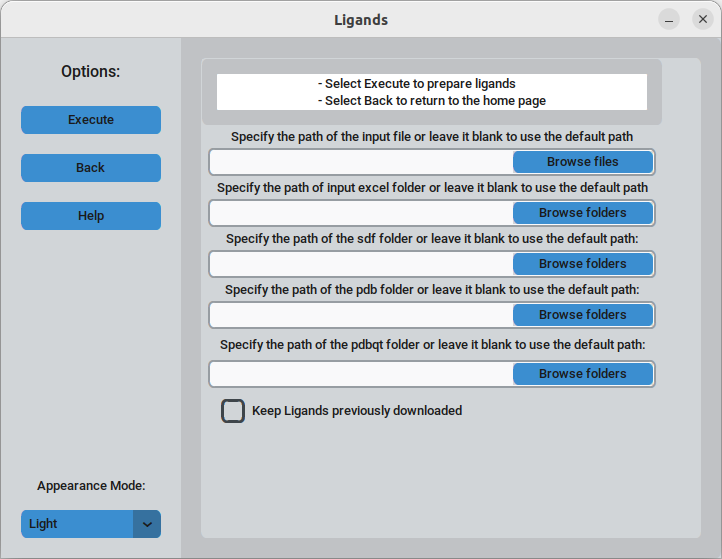
\includegraphics[scale=0.6]{immagini/capitolo3/ligands.png}
    \caption{Sezione Ligands della GUI}
    \label{fig:ligands}
\end{figure}

\begin{figure}[H]
    \centering
    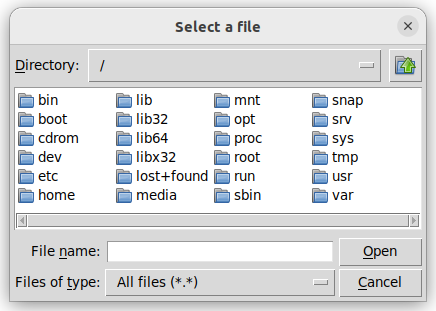
\includegraphics{immagini/capitolo3/browseFilesLigands.png}
    \caption{Browse files}
    \label{fig:browse files ligands}
\end{figure}

\begin{figure}[H]
    \centering
    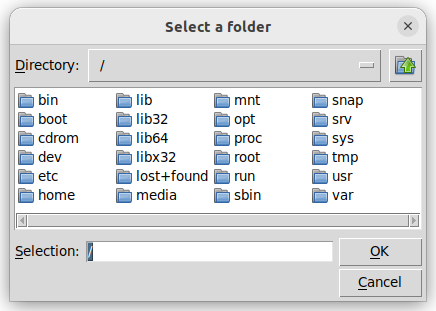
\includegraphics{immagini/capitolo3/browseFoldersLigands.png}
    \caption{Browse folders}
    \label{fig:browse folders ligands}
\end{figure}

La GUI per la preparazione dei ligandi richiama lo script \textbf{prepare\_ligands.py} discusso nella precedente sezione, adattando l'interfaccia grafica allo script senza eliminare alcuna funzionalità, precedentemente illustrata, per la versione da riga di comando e rispettando i dettami dell'\textbf{OOP}.\newline
Durante l'esecuzione viene mostrato un \textbf{pannello} (\ref{fig:ligands execution}) in cui vengono descritte:
\begin{itemize}
    \item le operazioni che si stanno effettuando
    \item eventuali errori ed avvisi per l'utente, in modo tale che sia restituito un feedback all'utente relativo al progresso della preparazione dei ligandi.
\end{itemize}
Al completamento di ogni fase sarà restituito un messaggio di avviso (figura: \ref{fig:progress completed ligands}) ed in caso di input non valido sarà restituito un messaggio di errore (figura: \ref{fig:invalid input ligands}).

\begin{figure}[H]
    \centering
    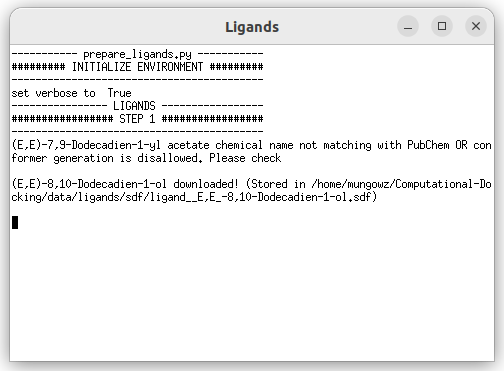
\includegraphics[scale=0.8]{immagini/capitolo3/ligandsExecution.png}
    \caption{Pannello dell'esecuzione dei ligandi}
    \label{fig:ligands execution}
\end{figure}

\begin{figure}[H]
    \centering
    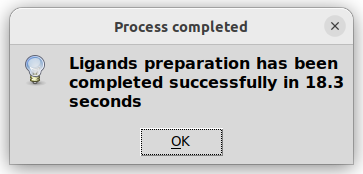
\includegraphics{immagini/capitolo3/progressCompletedLigands.png}
    \caption{Messaggio relativo al completamento della preparazione dei ligandi}
    \label{fig:progress completed ligands}
\end{figure}

\begin{figure}[H]
    \centering
    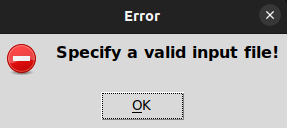
\includegraphics{immagini/capitolo3/invalidInputLigands.png}
    \caption{Messaggio di errore}
    \label{fig:invalid input ligands}
\end{figure}

\subsection{Preparazione dei recettori tramite script} \label{Preparazione dei recettori script}
Lo script python \textbf{prepare\_receptors.py}, che esegue tale fase, viene eseguito da terminale mediante il comando:

\begin{lstlisting}[language=Python, label=lst:code11, caption={funzione prepare\_receptors}]
python prepare_receptors.py
\end{lstlisting}

Questo script può ricevere diversi argomenti in input:

\begin{itemize}
    \item $[-v]$: serve per attivare il verbose e se non viene specificata tale opzione viene lasciata di default inattivo
    \item $[-E]$: specifica la directory dei file \textit{.xlsx} di output, se non viene specificata tale opzione verrà scelta la directory di default
    \item $[-P]$: specifica la directory dei file \textit{.pdb} di output, se non viene specificata tale opzione verrà scelta la directory di default
    \item $[-p]$: specifica la directory dei file \textit{.pdbqt} di output, se non viene specificata tale opzione verrà scelta la directory di default
    \item $[-k]$: specificando questa opzione viene scelto di non cancellare i file delle proteine precedentemente scaricati, se non viene specificata tale opzione i file verranno cancellati
    \item $[-m]$: specificando questa opzione viene fornita in input la dimensione in \textit{angstrom} del margine della \textit{grid box} per le proteine se non viene specificata tale opzione viene impostato il valore di default ovvero 3
    \item $[-h]$: stampa la spiegazione degli input per lo script.
\end{itemize}
Lo script quando eseguito andrà ad inizializzare i vari percorsi, nel caso siano stati inseriti percorsi diversi da quelli di default verrà controllata l'esistenza e la validità degli stessi. Nel caso non siano presenti le directory contenenti i file \textit{.txt}, \textit{.pdb} e \textit{.pdbqt}, queste verranno create automaticamente dall'applicazione, inoltre verranno cancellati i file precedentemente scaricati a meno di input diversi.\newline
Lo script richiama la funzione \textbf{selectReceptors} la quale si occupa di scaricare da \textbf{RCSB} i file \textit{.pdb} corrispondenti alle proteine scelte. La funzione prende in input: 

\begin{itemize}
    \item \textit{pdb\_folder}, il path della directory di output per i file \textit{.pdb}
    \item \textit{excel\_folder}, il path della directory di output per i file \textit{.xlsx}
    \item \textit{verbose}, il flag relativo al verbose.
\end{itemize}

In output sono restituiti i file \textit{.pdb} corrispondenti ai recettori scelti in input e un file \textit{.xlsx} contenente i risultati dell'operazione di download nominato \textit{info\_proteins.xls}.

\begin{lstlisting}[language=Python, label=lst:code12, caption={funzione selectReceptors}]
selectReceptors(pdb_folder, excel_folder, verbose)
\end{lstlisting}

All'interno di questa \textbf{selectReceptors} viene richiamata la funzione \textbf{RestApiSelection} la quale prende in input l'\textit{URL} di \href{https://www.rcsb.org/search}{RCSB}:

\begin{lstlisting}[language=Python, label=lst:code13, caption={funzione RestApiSelection}]
RestApiSelection(URL)
\end{lstlisting}

Questa funzione apre una \textbf{WebView} sul sito di \href{https://www.rcsb.org/search}{RCSB} come mostrato nella figura \ref{fig:query recettori}, l'utente potrà digitare la propria query e scaricare i composti scelti selezionando il tasto in alto \textbf{Get Query}.\newline
La \textbf{web view} restituisce l'\textbf{URL} della pagina del database contenente i composti selezionati dalla query, il \textit{JSON} di tale pagina viene estratto e convertito nella struttura dati \textit{dizionario} di python tramite la funzione \textbf{loads} della libreria \textbf{json}.

\begin{lstlisting}[language=Python, label=lst:code14, caption={funzione json.loads}]
dictionary = json.loads(data)
\end{lstlisting}

Nel \textit{dizionario} restituito dalla funzione sarà contenuto l'elenco dei composti selezionati tramite la query.\newline
Il software rieseguirà direttamente la query tramite la funzione \textbf{get} contenuta nella libreria \textbf{requests}. Questa funzione permette di inviare una richiesta di tipo \textit{HTTP/1.1} prendendo in input \textbf{URL} della query, al quale viene aggiunto l'elenco di composti da scegliere in formato \textit{JSON}, ciò eseguito convertendo il \textit{dizionario} precedentemente ottenuto in \textbf{JSON}
mediante la funzione \textbf{dump} della libreria \textbf{json}:

\begin{lstlisting}[language=Python, label=lst:code15, caption={funzione json.dump}]
dictionary = json.dump(dictionary)
\end{lstlisting}

La funzione \textbf{get} restituisce la lista di proteine da scaricare:

\begin{lstlisting}[language=Python, label=lst:code16, caption={funzione requests.get}]
requests.get(f"https://search.rcsb.org/rcsbsearch/v2/query?json={dictionary}")
\end{lstlisting}

La funzione \textbf{selectReceptors} richiama successivamente la funzione \textbf{downloadPdbs} che prende in input:

\begin{itemize}
    \item \textit{pdb\_list}, la lista di proteine precedentemente ottenuta
    \item \textit{outputh\_path}, il path della directory di output per i file \textit{.pdb}
    \item \textit{verbose}, il flag relativo al verbose.
\end{itemize}

La funzione restituisce in output i file \textit{.pdb} delle proteine contenute nella lista in input:

\begin{lstlisting}[language=Python, label=lst:code17, caption={funzione downloadPdbs}]
downloadPdbs(pdbs_list, output_path, verbose)
\end{lstlisting}

La funzione \textbf{downloadPdbs} richiama la funzione \textbf{fetchPDB} del pacchetto \textbf{ProDy}, che prende in input:

\begin{itemize}
    \item \textit{protein\_code}, la proteina da scaricare
    \item \textit{folder}, il path della directory di output per i file \textit{.pdb}, nel nostro caso sarà impostato ad \textit{out\_path}
    \item \textit{compressed}, il flag per decidere se il file scaricato dovrà essere compresso oppure no, nel nostro caso il flag sarà impostato a \textit{False} per indicare che i file scaricati debbano essere già decompressi.
\end{itemize}

Tramite tale istruzione è possibile interfacciarsi con \textbf{RCSB} e scaricare un singolo file \textit{.pdb} mediante richiesta \textit{FTP}, il download di tutte le proteine della lista avviene ciclando su tutti gli elementi di essa:

\begin{lstlisting}[language=Python, label=lst:code18, caption={funzione fetchPDB}]
fetchPDB(protein_code, folder=output_path, compressed=False)
\end{lstlisting}

Dopo aver effettuato il download di tutte i file \textit{.pdb} le informazioni relative al download ed ai file scaricati vengono salvati in un file \textit{.xlsx} chiamato \textit{info\_proteins.xlsx} che viene salvato nella directory \textit{/output/}.\newline
Lo script \textbf{prepare\_receptors.py} una volta terminata la funzione \textbf{selectReceptors} richiama la funzione \textbf{splitRepeatedResidues} che prende in input:

\begin{itemize}
    \item \textit{pdb\_folder}, il path della directory di output per i file \textit{.pdb}
    \item \textit{verbose}, il flag relativo al verbose.
\end{itemize}

Questa funzione si occupa di rimuovere i residui ripetuti memorizzati nel file \textit{.pdb} sotto la dicitura \textit{alternative location} o \textit{alt\_loc}:

\begin{lstlisting}[language=Python, label=lst:code19, caption={funzione splitRepeatedResidues}]
splitRepeatedResidues(pdb_folder, verbose, output_folder=None)    
\end{lstlisting}

Per accedere agli attributi dei file \textit{.pdb} utilizziamo la funzione \textbf{read\_pdb} del pacchetto \textbf{PandasPdb}, che prende in input il nome del file \textit{.pdb}:

\begin{lstlisting}[language=Python, label=lst:code20, caption={funzione PandasPdb.read\_pdb}]
PandasPdb.read_pdb(pdb_file)
\end{lstlisting}

Gli attributi ripetuti sono denominati \textit{A} e \textit{B}, di cui i \textit{B} saranno eliminati.\newline
Successivamente viene richiamata dallo script la funzione \textbf{deleteHeteroatomsChains}, la quale prende in input:

\begin{itemize}
    \item \textit{pdb\_folder}, il path della directory di output per i file \textit{.pdb}
    \item \textit{verbose}, il flag relativo al verbose.
\end{itemize}

Questa funzione si occupa di rimuovere le catene di eteroatomi contenute nel file \textit{.pdb}, queste sono evidenziate nel file tramite un loro attributo ovvero la keyword \textit{HETATM}, una volta rimosse, le catene vengono salvate. 

\begin{lstlisting}[language=Python, label=lst:code21, caption={funzione deleteHeteroatomsChains}]
deleteHeteroatomsChains(pdb_folder, verbose)
\end{lstlisting}

L'estrazione degli attributi dai file \textit{.pdb} avviene anche in questo caso tramite la funzione \textbf{read\_pdb} precedentemente descritta.\newline
Lo script \textbf{prepare\_receptors.py} richiama successivamente la funzione \textbf{splitChains} che prende in input: 

\begin{itemize}
    \item \textit{pdb\_folder}, il path della directory di output per i file \textit{.pdb}
    \item \textit{verbose}, il flag relativo al verbose.
\end{itemize}

Questa funzione si occupa di dividere le catene di residui che formano la struttura della proteina mantenendo soltanto le catene distinte, cioè quelle catene che hanno solo una sequenza amminoacidica distinta e non ripetuta da altre catene. 

\begin{lstlisting}[language=Python, label=lst:code22, caption={funzione splitChains}]
splitChains(pdb_folder, verbose)    
\end{lstlisting}

Tramite la funzione \textbf{parsePDB} della libreria \textbf{prody} viene ricostruita la struttura proteica attraverso i seguenti oggetti:

\begin{itemize}
    \item la lista delle molecole
    \item la lista degli atomi e dei residui, che viene rappresentata da un oggetto della classe \textbf{AtomGroup} restituito dalla funzione \textbf{parsePDB}.
\end{itemize}
, 

\begin{lstlisting}[language=Python, label=lst:code23, caption={funzione parsePDB}]
atoms = parsePDB(protein_file)
\end{lstlisting}

La ricostruzione della struttura proteica avviene tramite la vista gerarchica della struttura, ciò viene implementata tramite il metodo \textbf{getHierView} della classe \textbf{AtomGroup}:

\begin{lstlisting}[language=Python, label=lst:code24, caption={atoms.getHierVieW}]
atoms.getHierView()
\end{lstlisting}

Vengono quindi esaminate tutte le sequenze, sempre tramite la funzione \textbf{parsePDB}, e vengono scelte solo le sequenze distinte, infine vengono salvate in un file tutte le catene distinte come se fossero delle proteine attraverso la funzione \textbf{writePDB} di \textbf{prody}, che prende in input:

\begin{itemize}
    \item \textit{filename}, il nome del file
    \item \textit{new\_atoms}, il composto da salvare
\end{itemize}

Questi file prenderanno il nome della proteina principale al quale viene aggiunto un underscore (\textit{\_}) seguito dal nome della catena distinta salvata nel file.

\begin{lstlisting}[language=Python, label=lst:code25, caption={writePDB}]
writePDB(filename, new_atoms)
\end{lstlisting}

Lo step successivo nella preparazione dei recettori è effettuato dalla funzione \textbf{prepareReceptors}, che prende in input:

\begin{itemize}
    \item \textit{pdb\_folder}, la directory con i file \textit{.pdb} in input
    \item \textit{pdbqt\_folder}, la directory con i file \textit{.pdbqt} in output
    \item \textit{verbose}, il flag relativo al verbose
    \item \textit{charges\_to\_add}, la carica da aggiungere alle proteine.
\end{itemize}

La funzione restituisce la conversione in file \textit{.pdbqt} dei corrispondenti i file \textit{.pdb} dati in input.

\begin{lstlisting}[language=Python, label=lst:code26, caption={prepareReceptors}]
prepareReceptors(pdb_folder, pdbqt_folder, verbose)
\end{lstlisting}

La funzione \textbf{prepareReceptors} utilizza lo script \textbf{prepare\_receptors4} della suite \textbf{ADFR}. In realtà viene utilizzata una versione modificata di tale script: \textbf{replacePrepareReceptor4.sh}. Questa versione modificata tramite bash scripting sostituisce la carica di Gasteiger con la carica in input ovvero \textit{charges\_to\_add} che nel nostro caso sono cariche di Kollman come specificate dalla stringa \textit{"Kollman"}. Tramite questo script si effettua la corretta conversione da \textit{.pdb} a \textit{.pdbqt}. Lo script viene richiamato da riga di comando dalla funzione mediante il comando \textbf{prepare\_receptor}:

\begin{lstlisting}[language=bash, label=lst:code27, caption={comando per convertire file da .pdb a .pdbqt}]
prepare_receptor -r pdb_file_path -A checkhydrogens -C charges_to_add -e -o pdbqt_folder
\end{lstlisting}

Nell'istruzione sopra:

\begin{itemize}
    \item \textit{pdb\_file\_path} indica la directory con i file \textit{.pdb} in input ed è specificata tramite lo switch \textit{-r}
    \item \textit{checkydrogens} indica l'opzione tramite la quale vengono controllati gli atomi di idrogeno specificata lo switch \textit{-A}    
    \item \textit{charges\_to\_add} indica la carica usata in input impostata tramite lo switch \textit{-C} 
    \item \textit{pdbqt\_folder} indica la directory con i file \textit{.pdbqt} in output specificata tramite lo switch \textit{-o}
\end{itemize}

Tramite tale istruzione è possibile effettuare la conversione di un singolo file, mentre la conversione di tutti i \textit{.pdb} avviene ciclando su tutti i file nella directory corrispondente.\newline
L'ultima fase nella preparazione dei ligandi consiste nella creazione delle \textit{grid box}, mediante la funzione \textbf{createGridboxes} richiamata dallo script \textbf{prepare\_receptors.py}, la funzione prende in input:

\begin{itemize}
    \item \textbf{pdb\_folder}, la directory contenente i file \textit{.pdb} 
    \item \textbf{gridbox\_outputh\_folder}, la directory di output per le \textit{grid box}
    \item \textbf{margin}, la dimensione in \textit{angstrom} del margine della \textit{grid box}
    \item \textbf{verbose}, il flag relativo al verbose.
\end{itemize}

Per ogni proteina ottenuta deve essere creata una \textit{grid box}, che definisce lo spazio conformazionale dove si colloca la proteina, è definita da:

\begin{itemize}
    \item Un centro
    \item Le dimensioni
    \item L'esaustività, la quale sarà utilizzata da qualsiasi software da \textbf{AutoDock Vina} per la ricerca delle pose possibili del ligando.
\end{itemize}

Una \textit{grid box} definisce la regione delle proteine dove il docking viene effettuato. Qualsiasi altra regione al di fuori dalla \textit{grid box} non verrà presa in considerazione durante il processo di docking.\newline
Le \textit{grid box} sono un input richiesto da \textbf{AutoDock Vina} ma non da altri software per il docking.\newline

\begin{lstlisting}[language=Python, label=lst:code28, caption={createGridboxes}]
createGridboxes(pdb_folder, gridbox_output_folder, margin, verbose)
\end{lstlisting}

Per ogni proteina vengono estratti gli attributi contenuti nel proprio file e viene richiamata da \textbf{createGridboxes} la funzione \textbf{createGridbox}, questa prende in input: 

\begin{itemize}    
    \item \textbf{ppdb}, l'insieme di attributi del file \textit{.pdb} ottenuti come oggetto della classe \textbf{AtomGroup} restituito dalla funzione \textbf{parsePDB}
    \item \textbf{protein\_path}, il file \textit{.pdb} corrispondente ad una singola proteina
    \item \textbf{gridbox\_outputh\_folder}, la directory di output per le \textit{grid box}
    \item \textbf{margin}, la dimensione in \textit{angstrom} del margine della \textit{grid box}
    \item \textbf{verbose}, il flag relativo al verbose.
\end{itemize}

La funzione \textbf{createGridbox} costruisce una \textit{grid box} per una singola proteina utilizzando gli attributi del file \textit{.pdb} rispettando i parametri precedentemente definiti per una \textit{grid box}.

\begin{figure}
    \centering
    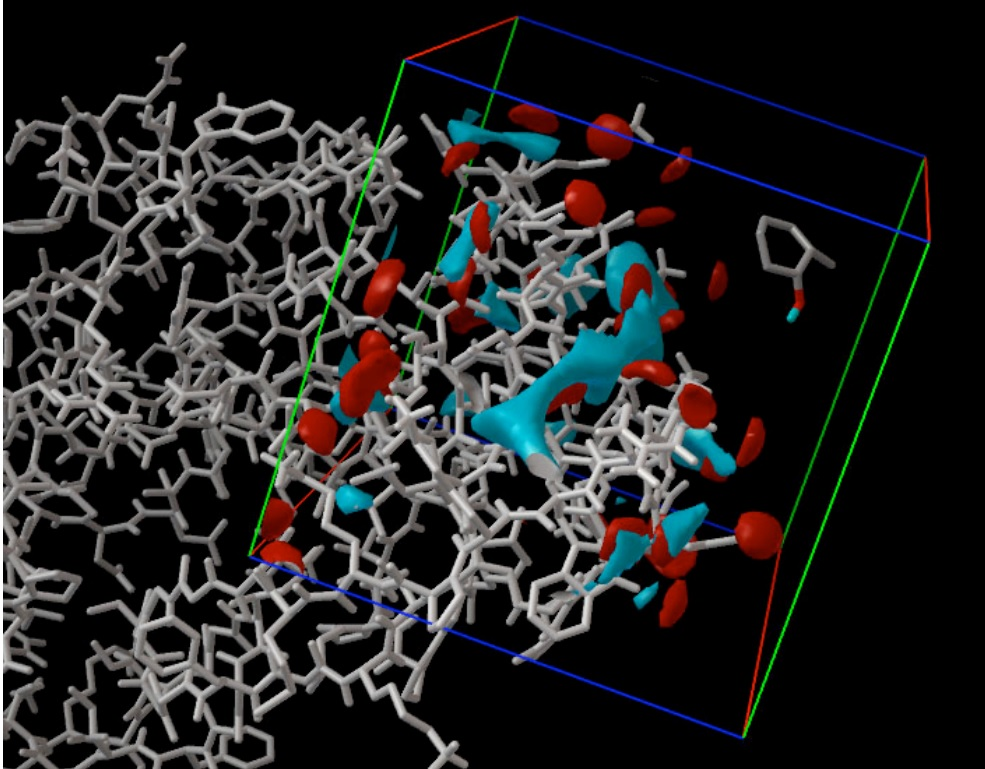
\includegraphics[scale=0.7]{immagini/capitolo3/gridbox.jpg}
    \caption{Gridbox mostrata all'interno della GUI di AutodockVina}
    \label{fig:gridbox}
\end{figure}

\subsection{Preparazione dei recettori tramite GUI}
La preparazione dei recettori tramite GUI avviene selezionando il tasto \textbf{Receptors} nella sezione \textbf{Preparation} del software. All'interno della pagina relativa alla preparazione dei recettori premendo il tasto \textbf{Execute} è possibile effettuare i procedimenti spiegati nella sezione relativa all'esecuzione tramite script (\ref{Preparazione dei recettori script}). Premendo il tasto \textbf{Back} è possibile tornare alla sezione \textbf{Preparation} relativa alla preparazione degli input.
Come si osserva nella figura \ref{fig:receptors} all'interno di tale sezione sono presenti delle \textbf{entry} dove è possibile specificare diversi input tra cui:

\begin{itemize}
    \item la directory dei file \textit{.xlsx} di output
    \item la directory dei file \textit{.pdb} di output
    \item la directory dei file \textit{.pdbqt} di output
    \item il valore del margine delle \textit{grid box}
\end{itemize}

Se lasciate vuote queste entry verrano impostate le configurazioni di default. E' presente anche un \textbf{checkbox} il quale se selezionato permette di mantenere i file precedentemente scaricati che altrimenti verrebbero cancellati.\newline
Per andare a selezionare direttamente nel file system del PC le directory richieste sono stati implementati i tasti \textbf{Browse folders}, come è visibile nelle figure \ref{fig:ligands} e \ref{fig:browse folders receptors}.

\begin{figure}[H]
    \centering
    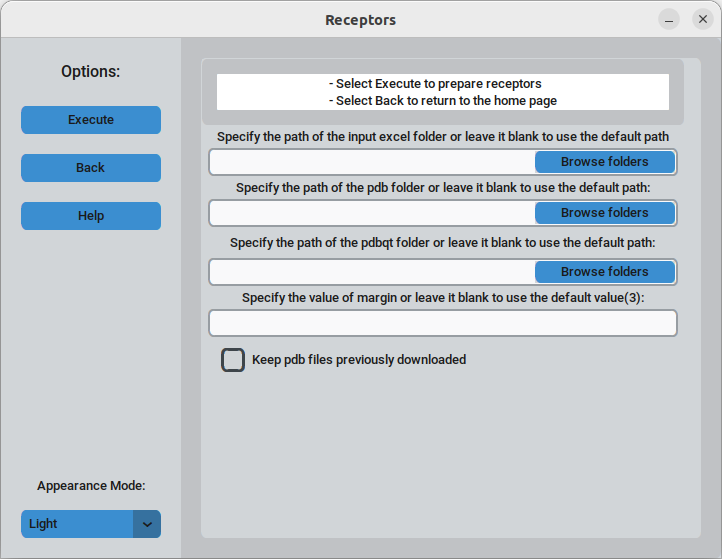
\includegraphics[scale=0.6]{immagini/capitolo3/receptors.png}
    \caption{Sezione Receptors della GUI}
    \label{fig:receptors}
\end{figure}

\begin{figure}[H]
    \centering
    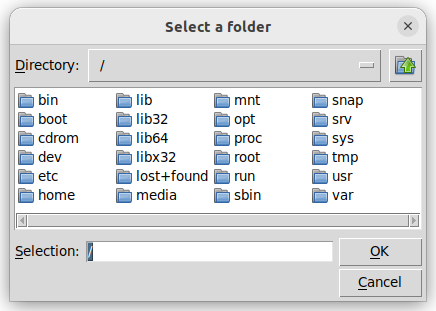
\includegraphics{immagini/capitolo3/browseFoldersReceptors.png}
    \caption{Browse folders}
    \label{fig:browse folders receptors}
\end{figure}

La GUI per la preparazione dei recettori richiama lo script \textbf{prepare\_receptors.py} discusso nella precedente sezione, adattando l'interfaccia grafica senza eliminare alcuna funzionalità della versione da riga di comando e rispettando i dettami dell'\textbf{OOP}.\newline
Durante l'esecuzione viene mostrato un \textbf{pannello} (\ref{fig:receptors execution}) in cui vengono descritti:

\begin{itemize}
    \item le operazioni che si stanno effettuando
    \item eventuali errori
    \item avvisi per l'utente.  
\end{itemize}

Tutto ciò per restituire un feedback all'utente relativo al progresso della preparazione dei recettori. Al completamento di ogni fase sarà restituito un messaggio di avviso (figura: \ref{fig:progress completed proteins}) ed in caso di input non valido sarà restituito un messaggio di errore (figura: \ref{fig:invalid input proteins}).

\begin{figure}[H]
    \centering
    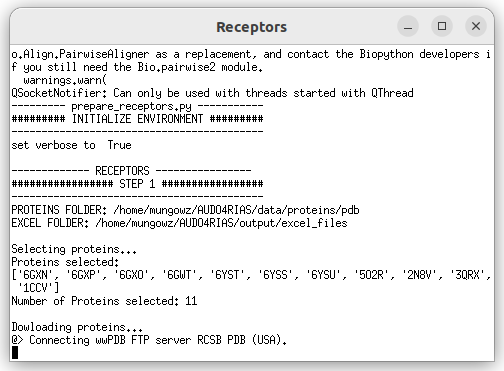
\includegraphics[scale=0.8]{immagini/capitolo3/receptorsExecution.png}
    \caption{Pannello dell'esecuzione dei recettori}
    \label{fig:receptors execution}
\end{figure}

\begin{figure}[H]
    \centering
    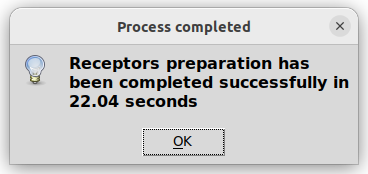
\includegraphics{immagini/capitolo3/progressCompletedReceptors.png}
    \caption{Messaggio relativo al completamento della preparazione dei ligandi}
    \label{fig:progress completed proteins}
\end{figure}

\begin{figure}[H]
    \centering
    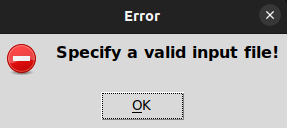
\includegraphics{immagini/capitolo3/invalidInputReceptors.png}
    \caption{Messaggio di errore}
    \label{fig:invalid input proteins}
\end{figure}

\section{Docking}
Il docking può essere considerato come l'operazione principale eseguita da \textbf{Computational Docking}. Il software scelto per eseguire il docking come detto in precedenza è \textbf{AutoDock Vina}, in particolare è stata scelta la versione 1.1.2 perchè dotata della capacità di produrre i file di log.\newline
La procedura del docking prende in input i dati ricavati dalla fase di preparazione precedentemente descritta. Risulta chiaro quindi come sia necessaria la corretta esecuzione della preparazione dei ligandi e delle proteine affinchè il docking vada a buon fine.

\subsection{Docking tramite script}
Dopo aver ottenuto i ligandi ed i recettori può essere effettuato il \textbf{Docking}, questo avviene mediante lo script bash \textbf{performDocking.sh}, il comando per eseguire lo script è:

\begin{lstlisting}[language=bash, label=lst:code29, caption={Comando per eseguire performDocking}]
./performDocking.sh -s vina
\end{lstlisting}

Lo script quando viene eseguito prende in input il parametro opzionale $-h$, che mostra il prompt con le istruzioni per l'uso dello script.\newline
Lo script prende in input la cartella dove sono presenti:

\begin{itemize}
    \item le proteine in formato \textit{.pdbqt}
    \item i ligandi in formato \textit{.pdbqt}
    \item le gridbox in formato \textit{.txt}
\end{itemize}

Successivamente verrà creata la cartella \textit{/output/docking} dove saranno salvati i risultati del docking e, per ogni coppia proteina-ligando verrà eseguito il seguente comando:

\begin{lstlisting}[language=bash, label=lst:code30, caption={Comando per eseguire il docking con Autodock Vina}]
vina --config gridbox_file.txt --receptor receptor_file.pdbqt --ligand ligand_file.pdbqt --out "{percorso_directory_software_installato}/output/docking/vina/cartella_nome_recettore/cartella_nome_ligando/out.pdbqt" --log "{percorso_directory_software_installato}/output/docking/vina/cartella_nome_recettore/cartella_nome_ligando/log.txt"
\end{lstlisting}

Nell'istruzione sopra:

\begin{itemize}
    \item \textit{Vina} è il commando per eseguire il docking con \textbf{AutoDock Vina}
    \item \textit{gridbox\_file.txt} è la gridbox in input relativa al recettore \textit{receptor\_file.pdbqt}, la gridbox è specificata dallo switch \textit{$--$config}
    \item \textit{receptor\_file.pdbqt} è il file di input del recettore nel formato \textit{.pdbqt}, specificato dallo switch \textit{$--$receptor}
    \item \textit{ligand\_file.pdbqt} è il file di input del ligando nel formato \textit{.pdbqt}, specificato dallo switch \textit{$--$ligand}
    \item \textit{directory di output}, specificata dallo switch \textit{$--$out}
    \item \textit{log di output}, specificato dallo switch \textit{$--$log}.
\end{itemize}

Questo comando è in grado di eseguire il docking per una sola coppia proteina-ligando. Per effettuare il docking su tutte le coppie deve essere eseguito tale comando per tutte le proteine su ogni ligando. Tale istruzione creerà una cartella per ogni proteina il cui nome corrisponde a quello della proteina (\textit{cartella\_nome\_recettore}), all'interno di tale cartella verranno create tante cartelle quanti sono i ligandi con cui vengono studiate le pose, il nome delle sottocartelle è quello dei rispettivi ligandi (\textit{cartella\_nome\_ligando}). All'interno di ogni sottocartella sono contenuti due file:

\begin{itemize}
    \item Un file \textit{.pdbqt} nominato out.pdbqt, il corrispondente output per la coppia proteina-ligando
    \item Un file \textit{.txt} nominato \textit{log.txt}, contenente le informazioni relative alla posa ottenuta. 
\end{itemize}

Se si considera la proteina \textbf{1fcu} ed il ligando \textbf{bentazone}, entrambi utilizzati nel caso di esempio, verrà creata una cartella nominata \textbf{1cfu} contenente una sottocartella nominata \textbf{bentazone} contenente a sua volta un file \textit{log.txt} e \textit{out.pdbqt}.

All'interno del file di log è possibile ricavare le seguenti informazioni:

\begin{itemize}
    \item \textit{mode}, il numero della posa calcolata in modo randomico
    \item \textit{affinity}, indica la stabilità del legame, misurata in kcal/mol, della coppia proteina-ligando ed è calcolata sul valore dell'energia di legame, più il valore è negativo o l'affinità di legame è bassa, più il ligando-recettore è stabile
    \item \textit{dist from best mode} indica la \textit{root-mean-square deviation (RMSD)} ossia la distanza media tra gli atomi, questo parametro si divide in due valori: \textit{lower bound (l. b)} distanza minima ed \textit{upper bound (u. p.)} distanza massima.
\end{itemize}

È possibile selezionare la migliore conformazione tra i risultati di \textbf{autoDock Vina}, ma non la migliore conformazione per una particolare proteina. Durante la ricerca delle pose il programma mantiene la conformazione data e inizia la selezione delle pose da lì. Per questo motivo si ottiene sempre un valore RMSD pari a 0. Di seguito il file di log del docking per la proteina \textbf{1fcu} combinata con il ligando \textbf{bentazone}:

\begin{figure}[H]
\begin{verbatim}
#################################################################
# If you used AutoDock Vina in your work, please cite:          #
#                                                               #
# O. Trott, A. J. Olson,                                        #
# AutoDock Vina: improving the speed and accuracy of docking    #
# with a new scoring function, efficient optimization and       #
# multithreading, Journal of Computational Chemistry 31 (2010)  #
# 455-461                                                       #
#                                                               #
# DOI 10.1002/jcc.21334                                         #
#                                                               #
# Please see http://vina.scripps.edu for more information.      #
#################################################################

WARNING: The search space volume > 27000 Angstrom^3 (See FAQ)
Detected 8 CPUs
Reading input ... done.
Setting up the scoring function ... done.
Analyzing the binding site ... done.
Using random seed: -2136627046
Performing search ... done.
Refining results ... done.

mode |   affinity | dist from best mode
     | (kcal/mol) | rmsd l.b.| rmsd u.b.
-----+------------+----------+----------
   1         -6.6      0.000      0.000
   2         -6.0      1.874      3.171
   3         -6.0     31.288     32.713
   4         -5.9     28.684     30.487
   5         -5.9     31.907     33.061
   6         -5.9     30.972     32.563
   7         -5.7      3.854      6.764
   8         -5.7      2.808      5.241
   9         -5.7     28.294     29.592
Writing output ... done.
\end{verbatim}
\caption{File di log del docking per la coppia proteina-ligando 1fcu-bentazone}
\label{fig:file di log}
\end{figure}

\subsection{Docking tramite GUI}
Il docking tramite GUI avviene selezionando il tasto \textbf{Docking} nella sezione \textbf{Home page} del software. All'inteno della pagina relativa al docking premendo il tasto \textbf{Execute} è possibile effettuare il docking, premendo il tasto \textbf{Back} è possibile tornare alla sezione \textbf{Home Page}.
Come si osserva nella figura \ref{fig:docking} all'interno di tale sezione sono presenti delle \textbf{entry} dove è possibile specificare diversi input tra cui:

\begin{itemize}
    \item la directory dei file \textit{.pdbqt} delle proteine di input
    \item la directory dei file \textit{.pdbqt} dei ligandi di input
    \item la directory dei file \textit{.txt} delle gridbox di input
    \item la directory dei log e dell'output del docking
\end{itemize}

Se lasciate vuote queste entry verrano impostate le configurazioni di default. E' presente anche un \textbf{checkbox} il quale se selezionato permette di mantenere i file precedentemente scaricati che altrimenti verrebbero cancellati.\newline
Per andare a selezionare direttamente nel file system del PC le directory richieste sono stati implementati i tasti \textbf{Browse folders}, come è visibile nelle figure \ref{fig:docking} e \ref{fig:browse folder docking}.

\begin{figure}[H]
    \centering
    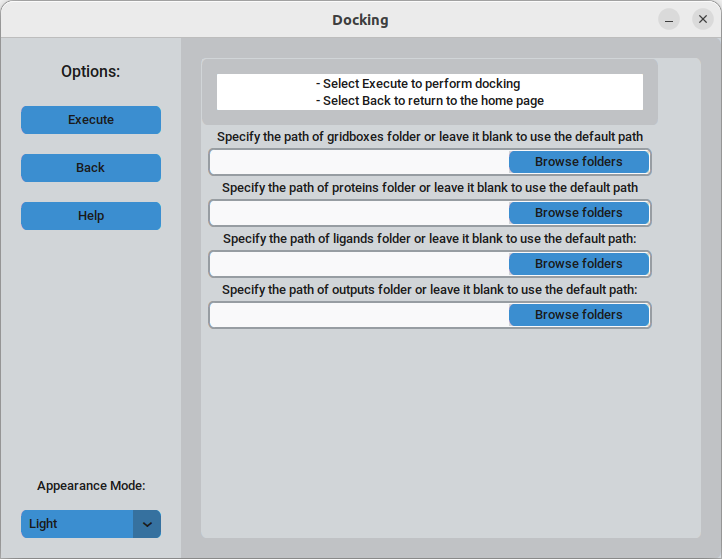
\includegraphics[scale=0.6]{immagini/capitolo3/docking.png}
    \caption{Sezione Docking della GUI}
    \label{fig:docking}
\end{figure}

\begin{figure}[H]
    \centering
    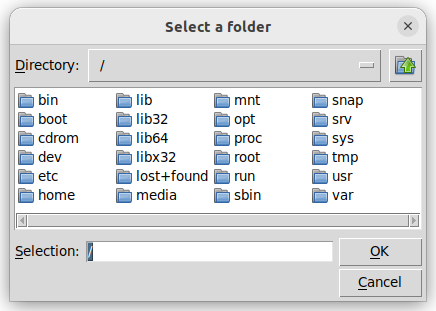
\includegraphics{immagini/capitolo3/browseFoldersDocking.png}
    \caption{Browse folder}
    \label{fig:browse folder docking}
\end{figure}

La GUI per il \textbf{docking} richiama lo script \textbf{performDocking.sh} discusso nella precedente sezione, adattando l'interfaccia grafica ad esso senza eliminare alcuna funzionalità precedentemente illustrata per la versione da riga di comando e rispettando i dettami dell'\textbf{OOP}.\newline
Durante l'esecuzione viene mostrato un \textbf{pannello} (\ref{fig:docking execution}) in cui vengono descritti: 

\begin{itemize}
    \item le operazioni che si stanno effettuando
    \item eventuali errori
    \item avvisi per l'utente.  
\end{itemize}

Tutto questo per restituire un feedback all'utente relativo al progresso del docking. Al completamento di ogni fase sarà restituito un messaggio di avviso (figura: \ref{fig:progress completed docking}) ed in caso di input non valido sarà restituito un messaggio di errore (figura: \ref{fig:invalid input docking}).

\begin{figure}[H]
    \centering
    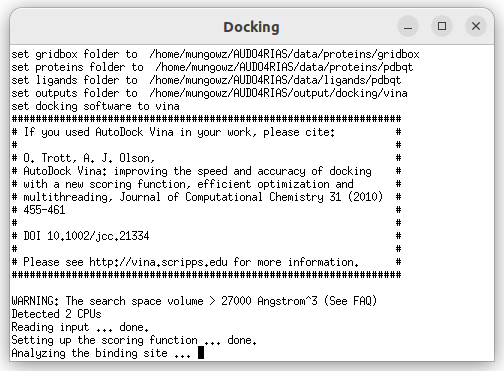
\includegraphics[scale=0.8]{immagini/capitolo3/dockingExecution.png}
    \caption{Pannello dell'esecuzione del docking}
    \label{fig:docking execution}
\end{figure}

\begin{figure}[H]
    \centering
    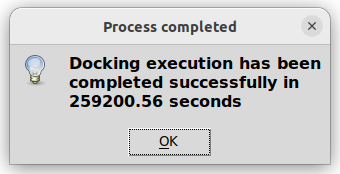
\includegraphics{immagini/capitolo3/progressCompletedDocking.png}
    \caption{Messaggio relativo al completamento dell' esecuzione del docking}
    \label{fig:progress completed docking}
\end{figure}

\begin{figure}[H]
    \centering
    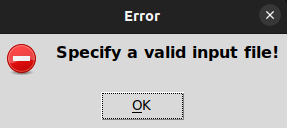
\includegraphics{immagini/capitolo3/invalidInputDocking.png}
    \caption{Messaggio di errore}
    \label{fig:invalid input docking}
\end{figure}

\section{Analisi}
Il processo di analisi consiste nell'analizzare l'output del docking per andare a determinare le interazioni (legami) presenti nelle pose ottenute. Le interazioni ricercate dal software sono:

\begin{itemize}
    \item I close-contacts
    \item Legami ad idrogeno
\end{itemize}


\subsection{Analisi tramite script}
L'analisi si divide in un primo step fondamentale che consiste nella rilevazione legami presenti all'interno delle pose risultanti dal docking, per implementare ciò è stato preso spunto dalla funzionalità messa a disposizione da \textbf{AutodockTools}. A seguito di un'ispezione fatta sul suo codice sorgente si è determinato che non è possibile richiamare le funzioni capaci di identificare i legami delle pose, per cui il loro codice sorgente è stato importato ed adattato al software trattato, lo script contenente queste funzioni e che si occupa della rilevazione delle interazioni è lo script python \textbf{detect\_interactions.py}.\newline
Il comando da digitare per eseguire l'analisi è:

\begin{lstlisting}[language=bash, label=lst:code31, caption={Comando per eseguire l'analisi}]
python3 detect_interactions.py
\end{lstlisting}

Lo script prende in input ciascun risultato del docking e restituisce: 

\begin{itemize}
    \item Un dizionario contenente le interazioni per ogni coppia-proteina ligando
    \item Il dizionario delle proteine dove per ciascun residuo e per ciascuna proteina coinvolti nelle interazioni, vengono memorizzati il numero di close-contacts ed il numero di legami ad idrogeno, questo dizionario è il risultato della fusione di tutti i dizionari delle coppie proteina-ligando
    \item Un dizionario contenente l'informazione relativa ai ligandi coinvolti nel calcolo dei residui, nello specifico viene salvato il tipo di ligando ed il tipo di interazione che si viene a formare nella coppia proteina-ligando. 
\end{itemize}

Il dizionario delle proteine e dei ligandi vengono serializzati e memorizzati come file binari.\newline
Le informazioni contenute in questi file vengono mostrate tramite heatmap e grafici a barre, questi vengono costruite tramite le funzioni di \textbf{numpy}.\newline
Le heatmap contengono sull'asse delle ascisse i ligandi e sull'asse delle ordinate i residui, ciascuna entry ligando-residuo può assumere tre stati:

\begin{itemize}
    \item Nessun legame, in viola
    \item Close-contact, in azzurro
    \item Legame ad idrogeno, in giallo 
\end{itemize}

Per mostrare l'heatmap di una singola proteina, salviamo solo il dizionario di una singola proteina anzichè il dizionario completo.\newline

\begin{figure}[H]
    \centering
    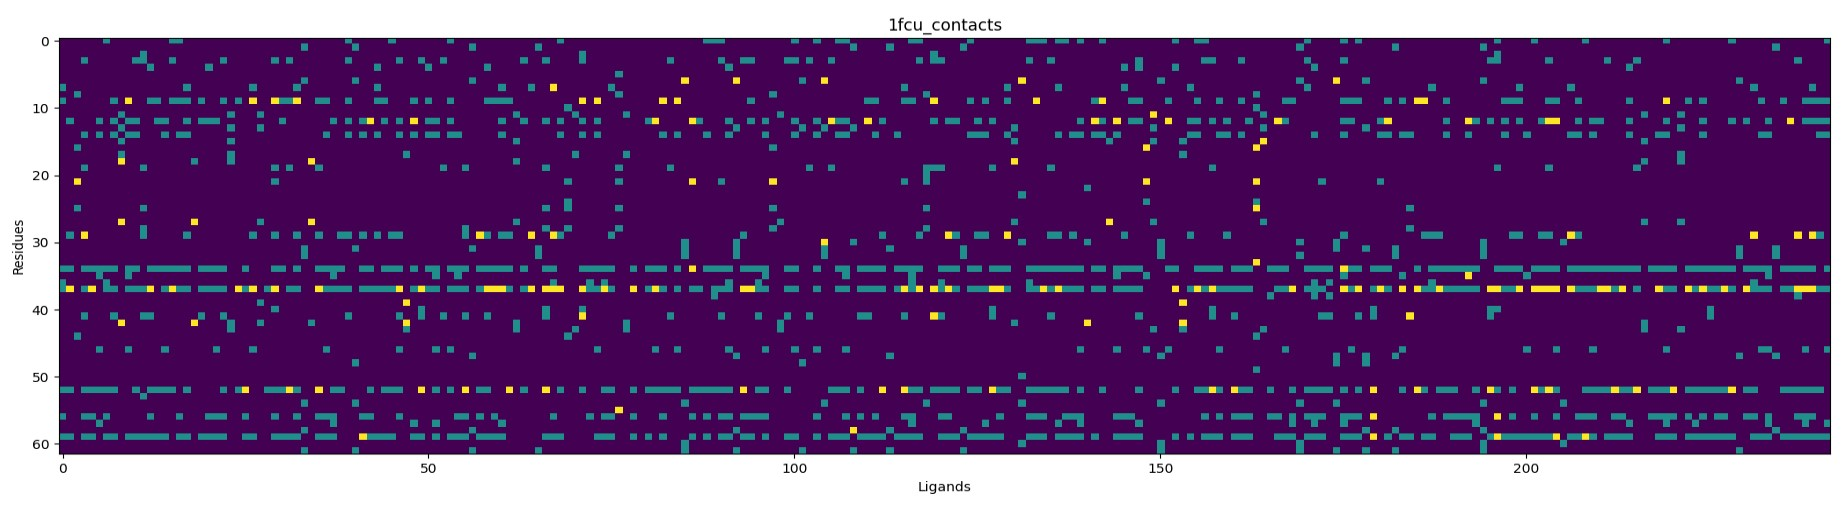
\includegraphics[scale=0.4]{immagini/capitolo3/heatmap.jpg}
    \caption{Heatmap relativa al residuo 1cfu}
    \label{fig:heatmap}
\end{figure}

I grafici a barre presentano sull'asse delle ascisse i residui e sull'asse delle ordinate il numero di legami e per ciascun residuo viene creata una barra stacked rappresentante il numero di close-contacts in blu ed il numero di legami ad idrogeno in giallo.

\begin{figure}[H]
    \centering
    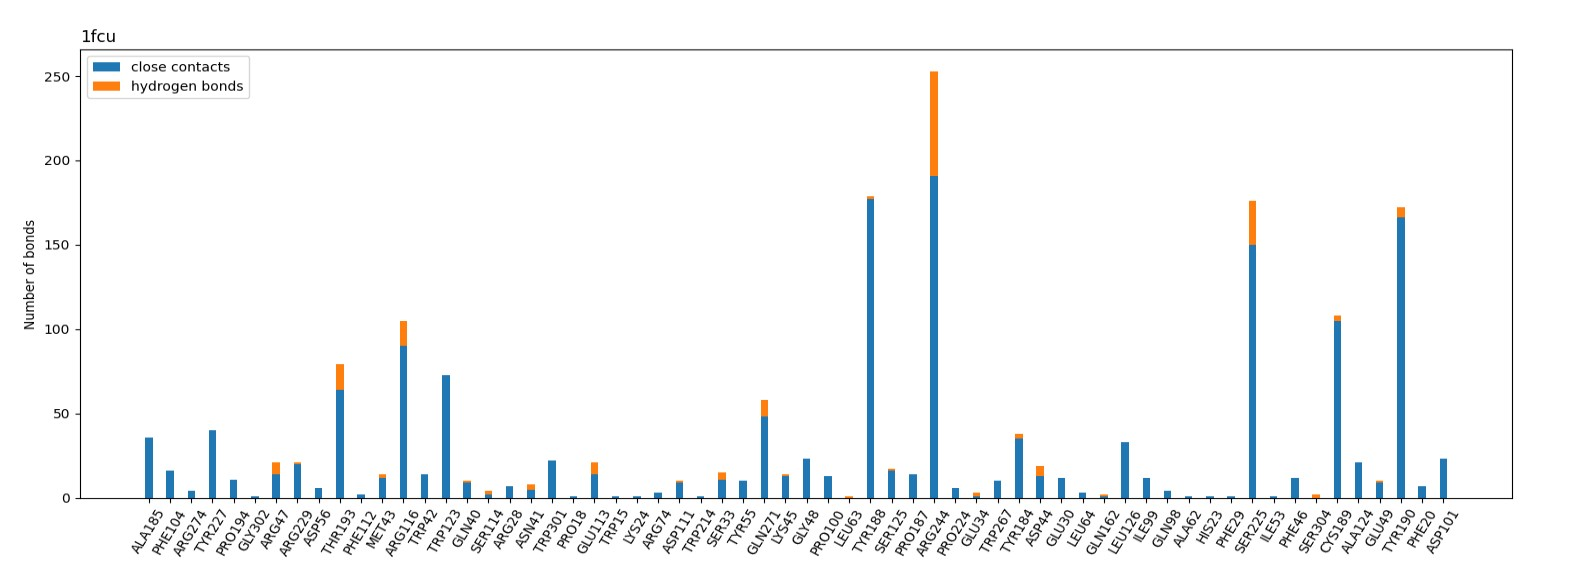
\includegraphics[scale=0.5]{immagini/capitolo3/interactions.jpg}
    \caption{Grafico a barre relativo al residuo 1cfu}
    \label{fig:interactions}
\end{figure}

\section{Analisi tramite GUI}
l'Analisi tramite GUI avviene selezionando il tasto \textbf{Analysis} nella sezione \textbf{Home page} del software. All'inteno della pagina relativa all'analisi premendo il tasto \textbf{Execute} è possibile effettuare l'analisi, premendo il tasto \textbf{Back} è possibile tornare alla sezione \textbf{Home Page}.

\begin{figure}[H]
    \centering
    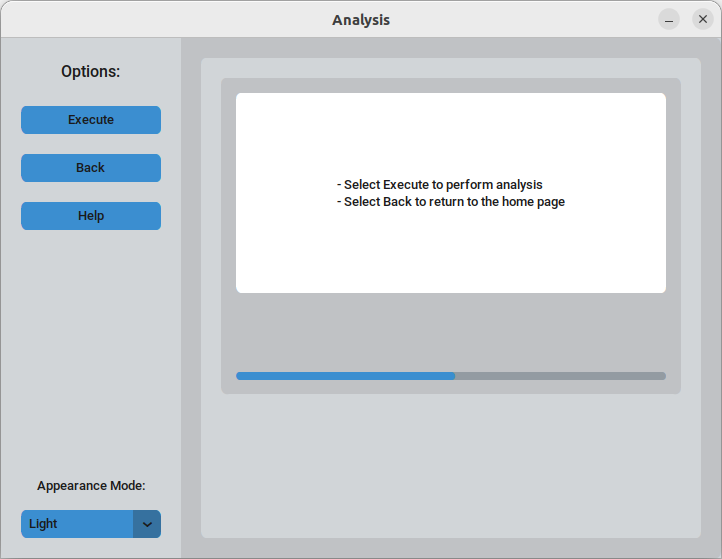
\includegraphics[scale=0.6]{immagini/capitolo3/analysis.png}
    \caption{Sezione Analysis della GUI}
    \label{fig:analisys}
\end{figure}

La GUI per l' \textbf{analisi} richiama lo script \textbf{detetct\_interactions.py} discusso nella precedente sezione, adattando l'interfaccia grafica ad esso senza eliminare alcuna funzionalità precedentemente illustrata per la versione da riga di comando e rispettando i dettami dell'\textbf{OOP}.\newline
Durante l'esecuzione viene mostrato un \textbf{pannello} (\ref{fig:analysis execution}) in cui vengono descritti: 

\begin{itemize} 
    \item le operazioni che si stanno effettuando
    \item eventuali errori
    \item avvisi per l'utente.  
\end{itemize}

Tutto questo per restituire un feedback all'utente relativo al progresso del analisi. Al completamento di ogni fase sarà restituito un messaggio di avviso (figura: \ref{fig:progress completed analysis}).

\begin{figure}[H]
    \centering
    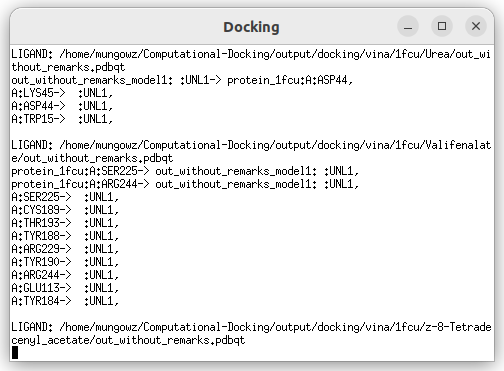
\includegraphics[scale=0.8]{immagini/capitolo3/analysisExecution.png}
    \caption{Pannello dell'esecuzione del analisi}
    \label{fig:analysis execution}
\end{figure}

\begin{figure}[H]
    \centering
    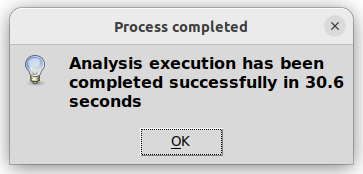
\includegraphics{immagini/capitolo3/progressCompletedAnalysis.png}
    \caption{Messaggio relativo al completamento dell'esecuzione dell'analisi con successo}
    \label{fig:progress completed analysis}
\end{figure}
    \chapter{Risultati sperimentali}
Per valutare le performance delle funzioni sviluppate, sono stati eseguiti 10 cicli incrementali per ciascuna funzionalità sviluppata, eccezion fatta per il docking la cui esecuzione con tutti i dati di input (289 ligandi, 11 recettori) presi in esame ha richiesto circa 3 giorni di esecuzione.\newline
Tutti i test sono stati eseguiti su \href{https://colab.research.google.com/}{Google Colaboratory} (Colab). Colab è una piattaforma gratuita che permette a chiunque di scrivere ed eseguire codice Python attraverso un browser. L’unico requisito è possedere un account Google (ad esempio Gmail). Colab è basato su un progetto Open Source chiamato \href{https://jupyter.org/}{Jupyter}. I documenti/programmi scritti su Colab sono chiamati Notebook e verranno salvati automaticamente sul Google Drive associato al proprio account.\newline
Le macchine virtuali messe a disposizione in Google Colab ospitano un ambiente configurato che consente di concentrarsi sin da subito sui progetti di Data Science:  sono presenti numerose librerie Python, tra cui moltissime di Data Science, si può usufruire di GPU e TPU per dare boost computazionali importanti ai lavori.\newline
Per facilitare la comprensione dei risultati ottenuti sono stati realizzati dei grafici, uno per ciascuna funzionalità testata.\newline
Ogni grafico riporta l'andamento dei tempi in funzione dell'incremento degli input relativi.\newline
Di seguito sono riportati i grafici relativi ai test effettuati per le funzioni:
\begin{itemize}
    \item Preparazione dei ligandi
    \item Preparazione dei recettori
    \item Esecuzione dell'analisi.
\end{itemize}

\begin{figure}[H]
    \centering
    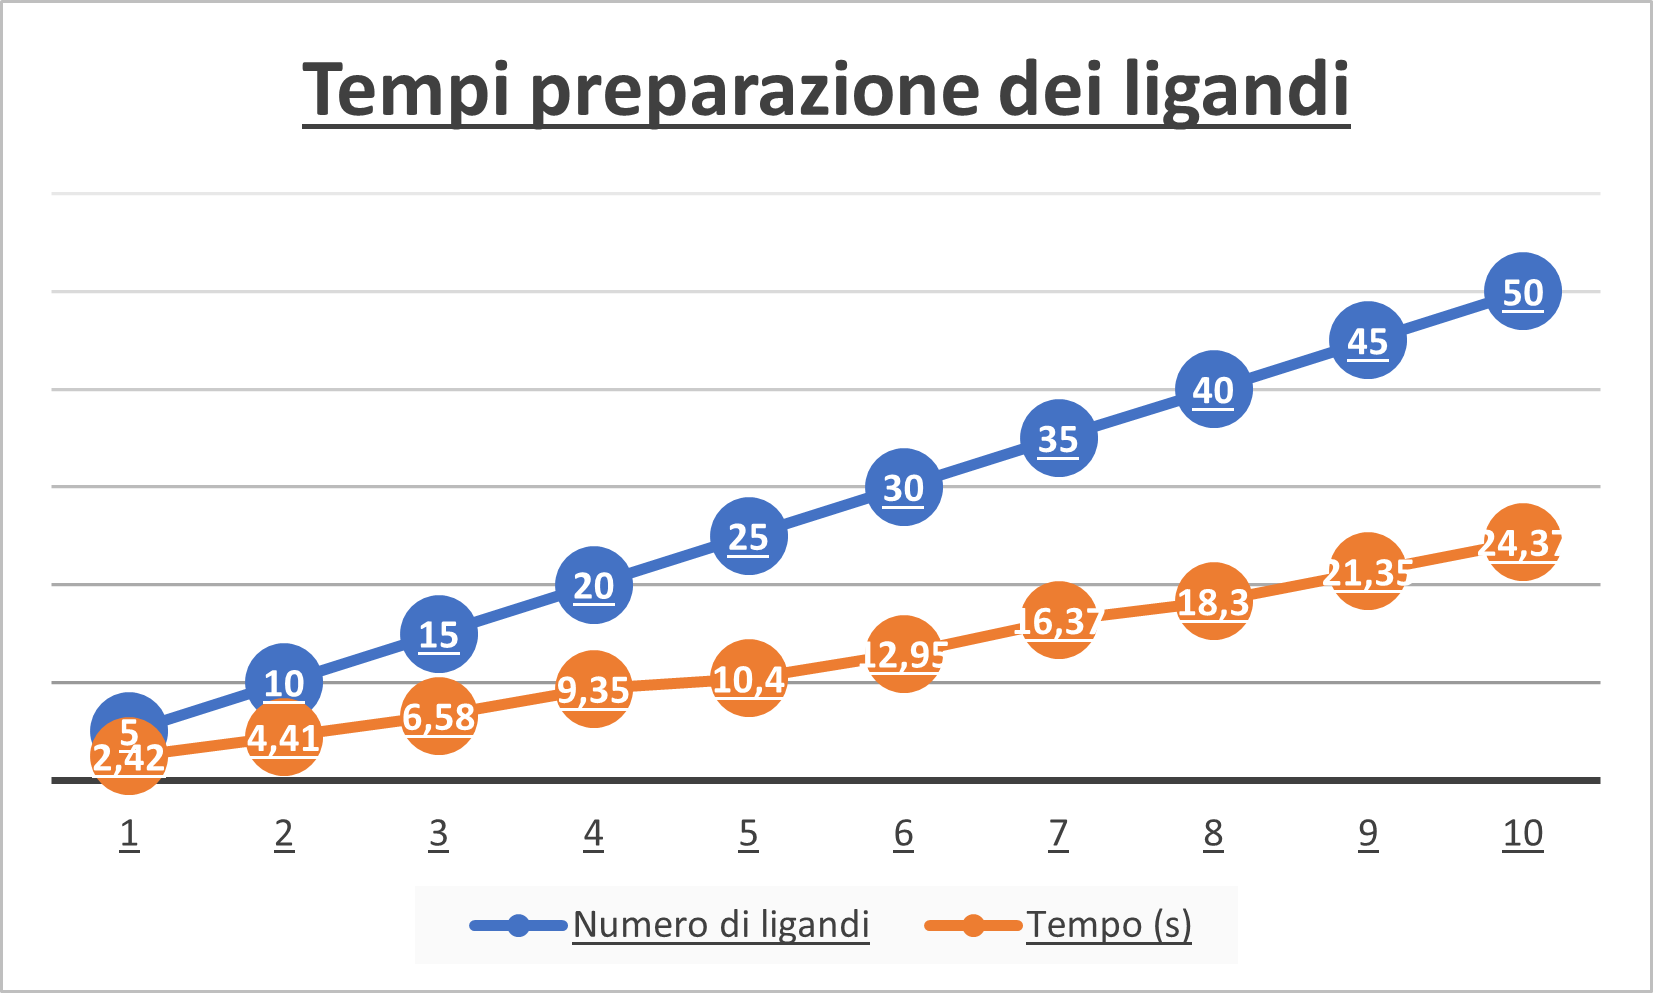
\includegraphics{immagini/capitolo4/tempiLigandi.png}
    \caption{Tempi di preparazione dei ligandi}
    \label{fig:tempi ligandi}
\end{figure}

\begin{figure}[H]
    \centering
    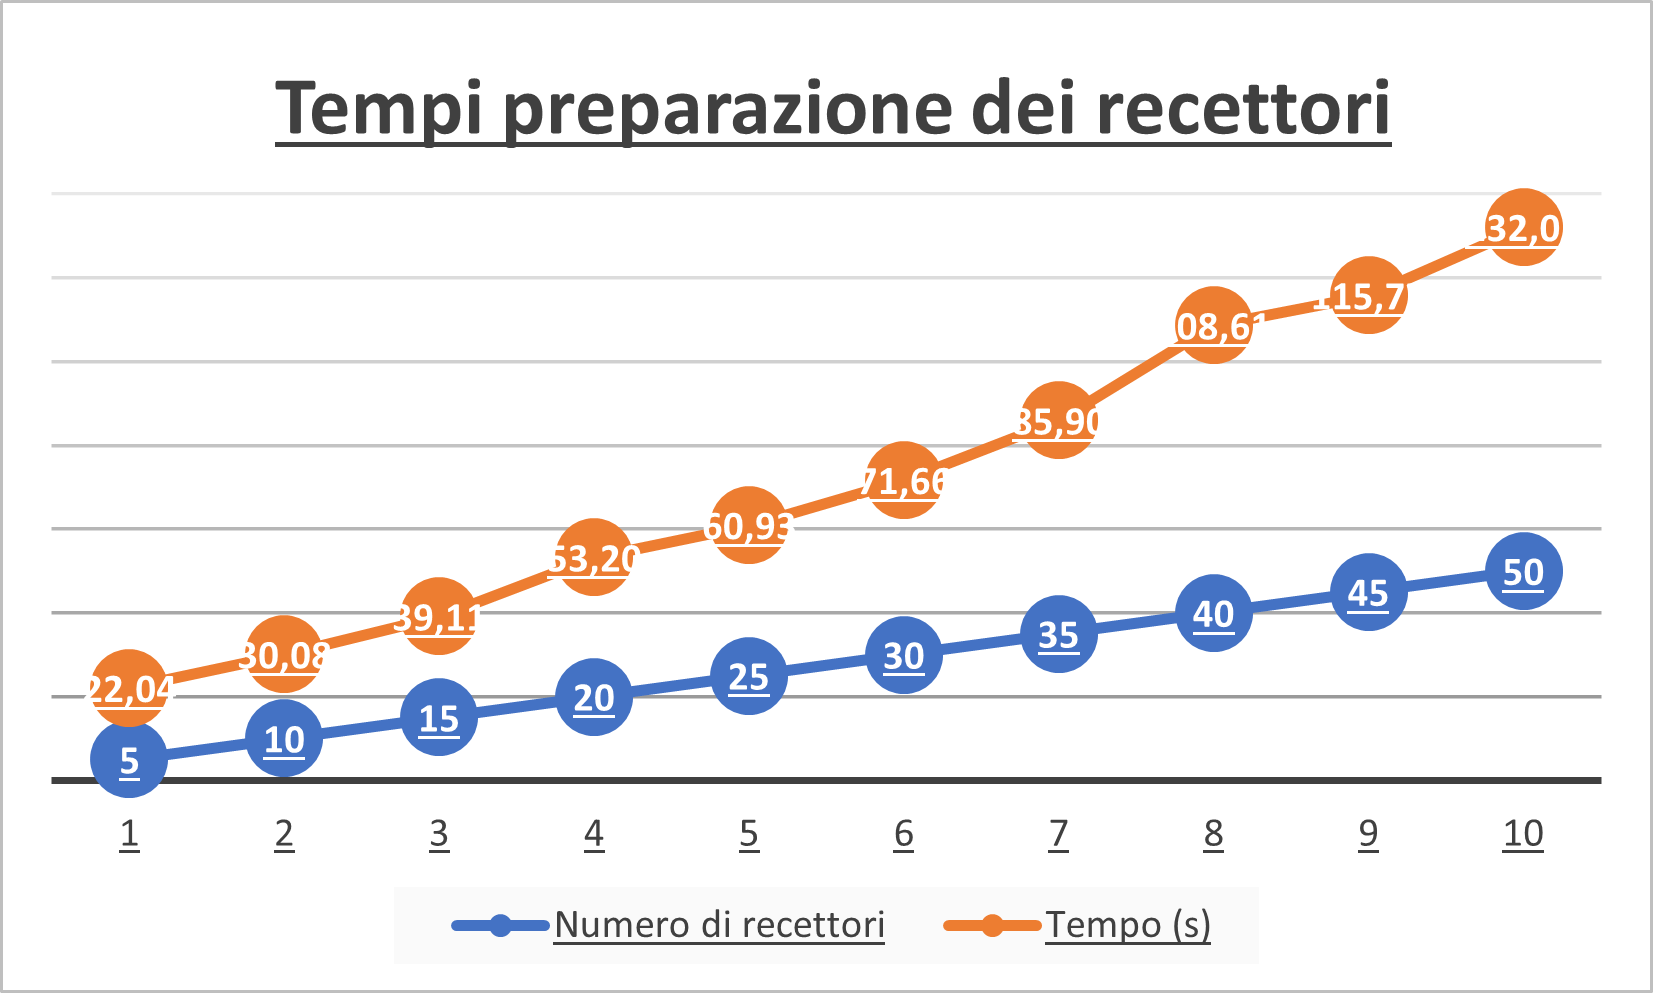
\includegraphics{immagini/capitolo4/tempiRecettori.png}
    \caption{Tempi di preparazione dei recettori}
    \label{fig:tempi recettori}
\end{figure}

\begin{figure}[H]
    \centering
    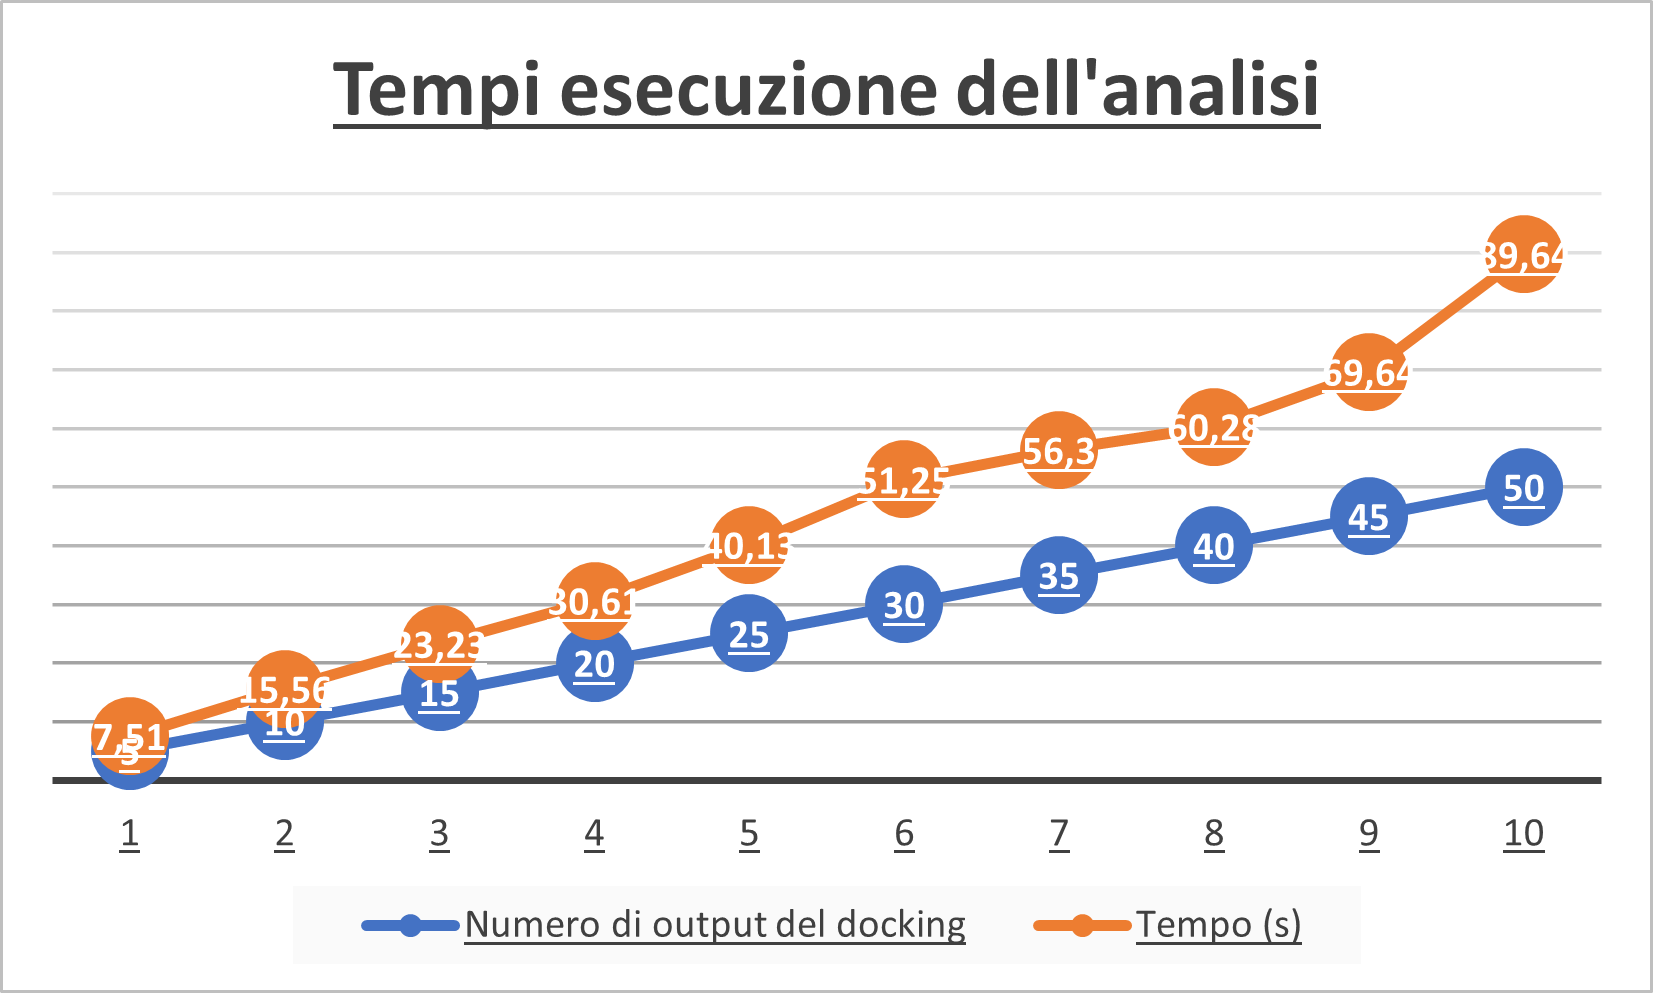
\includegraphics{immagini/capitolo4/tempiAnalisi.png}
    \caption{Tempi di esecuzione dell'analisi}
    \label{fig:tempi analisi}
\end{figure}

Osservando e comparando i dati dei grafici sopra, si può notare che:

\begin{itemize}
    \item le prestazioni delle funzioni, preparazione ligandi, preparazione recettori e analisi rispecchiano la stessa complessità di tempo
    \item le prestazioni del sistema in generale non degradano con il crescere dei dati in input
    \item l'andamento dei tempi si incrementa linearmente con l'aumentare dell'input.
\end{itemize}
    \chapter{Conclusioni e sviluppi futuri}
Nell'idea iniziale del progetto \textbf{Computational Docking} gli obbiettivi erano quelli di creare un software capace di automatizzare i processi di preparazione degli input per il docking, di esecuzione del docking e l'analisi dei suoi risultati, riunendo in una sola applicazione diverse funzioni e strumenti di bioInformatica. Raggiunti gli obbiettivi di cui sopra si è deciso di dotare il software prodotto di un'interfaccia grafica, per permettere anche a chi non abbia particolari conoscenze informatiche e familiarità con l'uso della riga di comando, di utilizzare l'applicazione in modo intuitivo, inoltre sono state aggiunte ulteriori funzionalità al software quali:

\begin{itemize}
    \item casi di analisi aggiuntivi
    \item altre opzioni di esecuzione. 
\end{itemize}

Il software descritto all'interno di tale documento ha la finalità di dare un apporto importante alla ricerca scientifica, in particolare è  progettato con lo scopo di analizzare dell'effetto dei pesticidi sull'Apis mellifera. Più nello specifico l'applicazione trattata ha più scopi: 

\begin{itemize}
    \item Riunire in un unico software tutti i tools e strumenti per effettuare il docking
    \item Fornire strumenti e procedure per l'analisi dei risultati del docking
    \item Automatizzare l'intero processo di docking e di analisi
    \item Dare la possibilità di sfruttare un'applicazione semplice, che non richiede particolari conoscenze in ambito informatico per l'utente finale.
\end{itemize}

\section{Conclusioni}
\textbf{Computational Docking} automatizza l'intero processo di screening biochimico partendo dalla preparazione dei \textbf{ligandi} e dei \textbf{recettori}, passando per il processo di \textbf{docking} e concludendo con l'analisi dell'output derivato dalla fase precedente.\newline
Viene concessa ampia libertà all'utente per quanto riguarda la scelta degli input e le impostazioni d'uso del software.
Il software realizzato, come si evince dai risultati sperimentali, è stato in grado di fornire risultati soddisfacenti dal punto di vista qualitativo, poichè sia i risultati del docking che l'analisi hanno soddisfatto i requisiti e le richieste del nostro esperto del dominio, il dottor Febbraio. Da un punto di vista quantitativo sono stati provati diversi output sia per tipo che per numero e l'applicazione è sempre stata in grado produrre risultati con tempistiche equiparabili ad altri software simili (Gold, Gnina, Keplero, ecc...).\newline
Un altro aspetto di cui si è tenuto conto è stata l'usabilità dell'applicazione, infatti \textbf{Computational Docking} è dotato di una \textbf{GUI} semplice da usare e che si avvicina non solo ai modelli di applicazione maggiormente diffusi sul mercato, facilitandone la comprensione da parte dell'utente, ma che gode di una buona responsività non solo nei confronti di chi la usa, il quale è sempre tenuto al corrente di ciò che il software stia facendo, ma anche per quanto riguarda i tempi di esecuzione, infatti tramite l'uso del parallelismo e della concorrenza sviluppati attraverso i thread, è possibile effettuare diversi compiti eseguiti dal software in parallelo e con tempi di risposta contenuti. E' bene ricordare che per andare incontro a macchine le quali non dispongono di molte risorse hardware è possibile utilizzare la versione da riga di comando del software, veloce e leggera.\newline
Inoltre l'applicazione è scalabile considerata la facilità di evoluzione per sviluppi futuri.
In conclusione \textbf{Computational Docking} è in grado di eseguire il docking, preparare i suoi input ed analizzarne gli output in maniera efficiente ed efficace.

\section{Sviluppi futuri}
Lo scopo dello sviluppo di \textbf{Computational Docking} è stato quello di analizzare gli effetti dei composti chimici contenuti all'interno dei pesticidi più diffusi, sulle api del genere Apis mellifera. L'obbiettivo a lungo termine dell'applicazione consiste nell'ampliare il suo dominio di analisi ad altre specie e casi, per esempio l'uomo, questo è l'obbiettivo ambizioso futuro per è progettato il software.\newline
Da un punto di vista puramente pratico una delle finalità principali dell'applicazione è quella di concedere sempre più libertà per quanto riguarda la modalità di input dei dati, nel caso specifico l'obbiettivo è quello di usare come banca dati non solo i database di \textbf{Pubchem} ed \textbf{RCSB}, ma usufruire anche degli altri archivi di composti chimici ed organici presenti in internet. Per quanto riguarda l'aspetto degli input sarebbe utile trovare una modalità di input per i \textbf{ligandi} simile a quella sfruttata per i \textbf{recettori}, garantendo una maggiore quantità di input da poter fornire.\newline
Da un punto di vista computazionale si mirerà ad usare pattern, strategie, algoritmi e schemi di programmazione che mireranno a ridurre sempre di più la complessità di tempo e spazio di \textbf{Computational Docking}.\newline
Detto ciò è chiaro come questo non sia un punto di arrivo ma un solo il punto di partenza del progetto \textbf{Computational Docking}.
    \appendix

\chapter{Tabella dei ligandi}
\begin{small}
    \begin{longtable}{|l|l|}
        \hline 
        (E,E)-7,9-Dodecadien-1-yl acetate & Gibberellins \\ \hline
        (E,E)-8,10-Dodecadien-1-ol & Glyphosate \\ \hline
        (3E,8Z,11Z)-Tetradeca-3,8,11-trienyl acetate & Halauxifen-methyl \\ \hline
        3E,8Z-Tetradecadienyl acetate & Halosulfuron-methyl \\ \hline
        (E)-11-Tetradecen-1-yl acetate & Hexythiazox \\ \hline
        (E)-5-Decen-1-ol & Hymexazol \\ \hline
        (E)-5-Decen-1-yl acetate & Imazalil \\ \hline
        (E)-8-Dodecen-1-yl acetate & Imazamox \\ \hline
        (Z,E)-7,11-Hexadecadien-1-yl acetate & Indolylbutyric acid \\ \hline
        (Z,E)-Tetradeca-9,11-dienyl acetate & Indoxacarb \\ \hline
        (Z,E)-9,12-Tetradecadien-1-yl acetate & Iodosulfuron \\ \hline
        (Z)-11-Hexadecen-1-ol & Ipconazole \\ \hline
        (Z)-11-Hexadecen-1-yl acetate & Iprovalicarb \\ \hline
        (Z)-11-Hexadecenal & Isofetamid \\ \hline
        (Z)-11-Tetradecen-1-yl acetate & Isopyrazam \\ \hline
        (Z)-13-Octadecenal & Isoxaben \\ \hline
        (Z)-7-Tetradecenal & Isoxaflutole \\ \hline
        (Z)-8-Dodecen-1-ol & Kresoxim-methyl \\ \hline
        (Z)-8-Dodecen-1-yl acetate & L-Ascorbic acid \\ \hline
        (Z)-8-Tetradecen-1-ol & lambda-Cyhalothrin \\ \hline
        z-8-Tetradecenyl acetate & Laminarin \\ \hline
        (Z)-9-Dodecen-1-yl acetate & Lauric acid \\ \hline
        (Z)-9-Hexadecenal & Lavandulyl senecioate \\ \hline
        (Z)-9-Tetradecen-1-yl acetate & Lenacil \\ \hline
        1-Decanol & Malathion \\ \hline
        1-methylcyclopropene & Maleic hydrazide \\ \hline
        1-Naphthylacetamide & Mandestrobin \\ \hline
        1-Naphthylacetic acid & Mandipropamid \\ \hline
        \multicolumn{2}{|r|}{{Continua nella pagina successiva}} \\ \hline
        1,4-Dimethylnaphthalene & MCPA \\ \hline
        2-Phenylphenol & MCPB \\ \hline
        2,4-D & Mecoprop-P \\ \hline
        Methyl 2,5-dichlorobenzoate & Mefentrifluconazole \\ \hline
        24-Epibrassinolide & Mepanipyrim \\ \hline
        4-(2,4-Dichlorophenoxy)butanoic acid & Mepiquat \\ \hline
        6-Benzyladenine & Meptyldinocap \\ \hline
        8-Hydroxyquinoline & Mesosulfuron \\ \hline
        Acequinocyl & Mesotrione \\ \hline
        Acetamiprid & Metaflumizone \\ \hline
        Acetic acid & Metalaxyl \\ \hline
        Acibenzolar-S-methyl & Metalaxyl-M \\ \hline
        Aclonifen & Metaldehyde \\ \hline
        Acrinathrin & Metam \\ \hline
        Ametoctradin & Metamitron \\ \hline
        Amidosulfuron & Metazachlor \\ \hline
        Aminopyralid & Metconazole \\ \hline
        Amisulbrom & Methoxyfenozide \\ \hline
        Azimsulfuron & Methyl decanoate \\ \hline
        Azoxystrobin & Methyl octanoate \\ \hline
        Beflubutamid & Zineb \\ \hline
        Benalaxyl-M & Metobromuron \\ \hline
        Benfluralin & Metrafenone \\ \hline
        Bensulfuron & Metribuzin \\ \hline
        Bentazone & Metsulfuron-methyl \\ \hline
        Benthiavalicarb & Milbemectin \\ \hline
        Benzoic acid & Tetradecyl acetate \\ \hline
        Benzovindiflupyr & Napropamide \\ \hline
        Bifenazate & Nicosulfuron \\ \hline
        Bifenox & Oleic acid \\ \hline
        Bispyribac & Orange oil \\ \hline
        Bixafen & Oxamyl \\ \hline
        Boscalid & Oxathiapiprolin \\ \hline
        Bromuconazole & Oxyfluorfen \\ \hline
        Bupirimate & Paclobutrazol \\ \hline
        Buprofezin & Pelargonic acid \\ \hline
        Capric acid & Penconazole \\ \hline
        Caprylic acid & Pendimethalin \\ \hline
        Captan & Penflufen \\ \hline
        Carfentrazone-ethyl & Penoxsulam \\ \hline
        Carvone & Penthiopyrad \\ \hline
        Chlorantraniliprole & Pethoxamid \\ \hline
        \multicolumn{2}{|r|}{{Continua nella pagina successiva}} \\ \hline
        Chlormequat & Phenmedipham \\ \hline
        Chlorotoluron & Phosmet \\ \hline
        Chromafenozide & Phosphane \\ \hline
        Clethodim & Picloram \\ \hline
        Clodinafop & Picolinafen \\ \hline
        Clofentezine & Pinoxaden \\ \hline
        Clomazone & Pirimicarb \\ \hline
        Clopyralid & Pirimiphos-methyl \\ \hline
        Cyantraniliprole & Potassium bicarbonate \\ \hline
        Cyazofamid & Prochloraz \\ \hline
        Cycloxydim & Prohexadione \\ \hline
        Cyflufenamid & Propamocarb \\ \hline
        Cyflumetofen & Propaquizafop \\ \hline
        Cyhalofop-butyl & Propoxycarbazone \\ \hline
        Cymoxanil & Propyzamide \\ \hline
        Cypermethrin & Proquinazid \\ \hline
        Cyprodinil & Prosulfocarb \\ \hline
        Daminozide & Prosulfuron \\ \hline
        Dazomet & Prothioconazole \\ \hline
        Deltamethrin & Pyraclostrobin \\ \hline
        Dicamba & Pyraflufen-ethyl \\ \hline
        Dichlorprop-P & Pyridaben \\ \hline
        Diclofop & Pyridalyl \\ \hline
        Difenoconazole & Pyridate \\ \hline
        Diflufenican & Pyrimethanil \\ \hline
        Dimethachlor & Pyriofenone \\ \hline
        Dimethenamid-P & Pyriproxyfen \\ \hline
        Dimethomorph & Pyroxsulam \\ \hline
        Dimoxystrobin & Quinmerac \\ \hline
        Dithianon & Quizalofop-P \\ \hline
        Dodecan-1-ol & Quizalofop-P-ethyl \\ \hline
        Dodecyl acetate & Quizalofop-P-tefuryl \\ \hline
        Dodemorph & Rescalure \\ \hline
        Dodine & Rimsulfuron \\ \hline
        Ethephon & S-Metolachlor \\ \hline
        Ethofumesate & Sedaxane \\ \hline
        Etofenprox & Sodium 2-methoxy-5-nitrophenolate \\ \hline
        Etoxazole & Sodium 2-nitrophenolate \\ \hline
        Eugenol & Sodium 4-nitrophenolate \\ \hline
        Fenazaquin & Spiromesifen \\ \hline
        Fenhexamid & Spirotetramat \\ \hline
        Fenoxaprop-P & Spiroxamine \\ \hline
        \multicolumn{2}{|r|}{{Continua nella pagina successiva}} \\ \hline
        Fenpicoxamid & Sulcotrione \\ \hline
        Fenpropidin & Sulfosulfuron \\ \hline
        Fenpyrazamine & Sulfoxaflor \\ \hline
        Fenpyroximate & Sulfuryl fluoride \\ \hline
        Flazasulfuron & tau-Fluvalinate \\ \hline
        Flonicamid & Tebuconazole \\ \hline
        Florasulam & Tebufenozide \\ \hline
        Florpyrauxifen-benzyl & Tebufenpyrad \\ \hline
        Fluazifop-P & Tefluthrin \\ \hline
        Fluazinam & Tembotrione \\ \hline
        Flubendiamide & Terbuthylazine \\ \hline
        Fludioxonil & Tetraconazole \\ \hline
        Flufenacet & Tetradecan-1-ol \\ \hline
        Flumetralin & Thiabendazole \\ \hline
        Flumioxazin & Thiencarbazone-methyl \\ \hline
        Fluometuron & Thifensulfuron-methyl \\ \hline
        Fluopicolide & Thymol \\ \hline
        Fluopyram & Tolclofos-methyl \\ \hline
        Fluoxastrobin & Tri-allate \\ \hline
        Flupyradifurone & Tribenuron \\ \hline
        Fluquinconazole & Triclopyr \\ \hline
        Flurochloridone & Trifloxystrobin \\ \hline
        Fluroxypyr & Triflusulfuron \\ \hline
        Flutianil & Trinexapac \\ \hline
        Flutolanil & Triticonazole \\ \hline
        Fluxapyroxad & Tritosulfuron \\ \hline
        Folpet & Urea \\ \hline
        Foramsulfuron & Valifenalate \\ \hline
        Forchlorfenuron & Ziram \\ \hline
        Formetanate & Zoxamide \\ \hline
        Fosetyl & Quartz sand \\ \hline
        Fosthiazate & Silthiofam \\ \hline
        Gamma-cyhalothrin & Esfenvalerate \\ \hline
        Garlic extract & Ethylene \\ \hline
        Geraniol & Gibberellic acid \\ \hline
        \multicolumn{2}{|r|}{{(2Z,4E)-5-[(1S)-1-Hydroxy-2,6,6-trimethyl-4-oxocyclohex-2-en-1-yl]-3-methylpenta-2,4-dienoic acid}}\\ \hline
        \multicolumn{2}{|r|}{{1-(4-Chlorophenyl)-5-(2-methoxyethoxy)-4-oxo-1,4-dihydrocinnoline-3-carboxylic acid}}\\ \hline
        \caption{Tabella dei ligandi in input} \label{tab:Tabella dei Ligandi}\\
    \end{longtable}
\end{small}

\chapter{Tabella dei recettori}
\begin{table}[!ht]
    \centering
    \begin{tabular}{|l|l|l|l|l|}
        \hline
        5YYL & 3BFA & 3D78 & 6LQK & 2MLT \\ \hline
        7ASD & 3BFB & 3FE6 & 6O4M & 2MW6 \\ \hline
        1BH1 & 3BFH & 3FE8 & 7OXF & 2N8V \\ \hline
        1CCV & 3BJH & 3FE9 & 7ZS6 & 3D75 \\ \hline
        1FCQ & 3CAB & 3R72 & 2J88 & 3D76 \\ \hline
        1FCU & 3CDN & 3RZS & 3QRX & 3D77 \\ \hline
        1FCV & 3CYZ & 3S0A & 6GXN & 5OHX \\ \hline
        1POC & 3CZ0 & 3S0B & 6GXP & 5XZ3 \\ \hline
        1TER & 3CZ1 & 3S0D & 4E81 & 6DST \\ \hline
        1TUJ & 3CZ2 & 3S0E & 6GXO & 6YSS \\ \hline
        2H8V & 3D73 & 3S0F & 6GWT & 6YSU \\ \hline
        2LIC & 3D74 & 3S0G & 6YST & 5O2R \\ \hline
    \end{tabular}
    \caption{Tabella dei recettori in input} 
    \label{Tabella dei Recettori}
\end{table}

    \nocite{*}
    \printbibliography[heading=bibintoc]

\end{document}